\documentclass[runningheads]{llncs}
%
\usepackage[numbers]{natbib}
\usepackage{url,bm}
\usepackage[breaklinks=true,unicode=true,urlcolor = blue,colorlinks = true,citecolor = blue,linkcolor = blue]{hyperref}
\usepackage{amssymb}
\usepackage{amsmath}
\setcounter{tocdepth}{3}
\usepackage{graphicx}
%
\graphicspath{{./figs/}}
%
\renewcommand\bibname{References}
%
\renewcommand{\vec}[1]{\bm{#1}}
% Define Authors
%
% 
\urldef{\mailsa}\path|{k.yershov@ifw-dresden.de,|
	\urldef{\mailsb}\path|o.volkov@hzdr.de}|   
\newcommand{\keywords}[1]{\par\addvspace\baselineskip
	\noindent\keywordname\enspace\ignorespaces#1}

\begin{document}
%\preprint{\textcolor[rgb]{0.00,0.50,0.75}{\texttt{Draft \gitAbbrevHash{} by \gitCommitterName{} on \gitCommitterIsoDate}}}	
	\mainmatter  % start of an individual contribution
	
	% first the title is needed
	\title{Flat curved systems}
	
	% a short form should be given in case it is too long for the running head
	\titlerunning{Flat curved systems}
	
	% the name(s) of the author(s) follow(s) next
	%
	% NB: Chinese authors should write their first names(s) in front of
	% their surnames. This ensures that the names appear correctly in
	% the running heads and the author index.
	%
	\author{Kostiantyn V. Yershov$^{1,2}$ \and Oleksii M. Volkov$^{3}$}
	%
	\authorrunning{Flat curved systems: Kostiantyn V. Yershov and Oleksii M. Volkov}
	% (feature abused for this document to repeat the title also on left hand pages)
	
	% the affiliations are given next; don't give your e-mail address
	% unless you accept that it will be published
	\institute{$^1$Bogolyubov Institute for Theoretical Physics of NAS of Ukraine,\\
		Metrologichna str. 14,  03143 Kyiv, Ukraine\\
		$^2$Leibniz-Institut f\"ur Festk\"orper- und Werkstoffforschung, IFW Dresden,\\
		 Helmholtzstra{\ss}e 20, D-01171 Dresden, Germany\\
		 $^{3}$Helmholtz-Zentrum Dresden-Rossendorf e. V. Institute of Ion Beam Physics and Materials Research,
		 Bautzner Landstra{\ss}e 400, 01328 Dresden, Germany\\
		\mailsa
		\mailsb}
	
	%
	% NB: a more complex sample for affiliations and the mapping to the
	% corresponding authors can be found in the file "llncs.dem"
	% (search for the string "\mainmatter" where a contribution starts).
	% "llncs.dem" accompanies the document class "llncs.cls".
	%
	
	\toctitle{Flat curved systems}
	\tocauthor{Kostiantyn V. Yershov and Oleksii M. Volkov}
	\maketitle
	
	
%\begin{abstract}
%	Abstract...
%	\keywords{Ferromagnets, curvilinear geometry, exchange interaction}
%\end{abstract}
	
\tableofcontents
\clearpage	

\section{Introduction}\label{sec:intro}

\section{Theory of flat curved systems}\label{sec:theory_1D}

\subsection{Model of curved 1D systems}\label{sec:model_1D}

The theoretical description of the evolution of the magnetization distribution in curved systems is based on the dynamics of the 3D vector order parameter $\vec{m}$ governed by the Landau--Lifshitz--Gilbert equation
\begin{equation}\label{eq:llg}
    \frac{\mathrm{d}\vec{m}}{\mathrm{d}t}=\underbrace{-\gamma_0\, \vec{m}\times\vec{H}_\textsc{eff}}_{\text{Precession term}} + \underbrace{\alpha_\textsc{g}\, \vec{m}\times\frac{\mathrm{d}\vec{m}}{\mathrm{d}t}}_{\text{Damping term}}.
\end{equation}
Here $\vec{m}=\vec{M}/M_s$ is a unit magnetization vector with $M_s$ being the saturation magnetization, $\alpha_\textsc{g}$ is the Gilbert damping parameter, $\gamma_0$ is a gyromagnetic ratio, and $\vec{H}_\textsc{eff}=-\delta E/\delta\vec{M}$ is an effective field with $E$ being the total energy of the magnet. The first term in~\eqref{eq:llg} describes the precession of the magnetization vector $\vec{m}$ around an effective field $\vec{H}_\textsc{eff}$, while the second term describes the damping of the  magnetization, i.e. as time passes, the magnetization spirals down until it becomes aligned with the field $\vec{H}_\textsc{eff}$.  We consider here a simple form of the energy of the magnet in the following form%  The phenomenological description of magnetization statics and dynamics in the continuum limit relies on the total energy of the magnet~(for the simplicity we consider uniaxial anisotropy)
\begin{equation}\label{eq:total_energy}
	E=\int\mathrm{d}V\left\{A\mathcal{E}_\textsc{e}+K\left[1-\left(\vec{m}\cdot\vec{e}_\textsc{a}\right)^2+\varepsilon\left(\vec{m}\cdot\vec{e}_\textsc{p}\right)^2\right]\right\}.
	%E=\int\mathrm{d}V\left\{A\mathcal{E}_\textsc{e}+K\left[1-\left(\vec{m}\cdot\vec{e}_\textsc{a}\right)^2+\varepsilon\left(\vec{m}\cdot\vec{e}_\textsc{p}\right)^2\right]+\mathcal{E}_\textsc{dm}\right\}.
\end{equation}
Here, the first term in~\eqref{eq:total_energy} describes the isotropic exchange interaction $\mathcal{E}_\textsc{e}=\sum_{i=x,y,z}\left(\vec{\nabla} m_i\right)^2$ with with the exchange stiffness $A$. The unit vectors $\vec{e}_\textsc{a}$ and $\vec{e}_\textsc{p}$ in Eq.~\eqref{eq:total_energy} gives the direction of the easy- and hard-axis anisotropy directions, respectively; $K>0$ is the easy-axial anisotropy constant and $\varepsilon>0$ is an anisotropy ratio. Such kind of anisotropy is effectively induced by the magnetostatic interaction in the thin stripes. In the curved ferromagnetic systems magnetostatic interaction can be reduced to the easy-tangential anisotropy for wires with circular/square cross-section~\cite{Slastikov12} or biaxial anisotropy with eassy-plane perpendicular to the wires plane for rectangular cross sections~\cite{Aharoni98,Gaididei17a}, which simply results in a shift of anisotropy constants. For thin, narrow, and curved stripes (ribbons) the approximation of the shape anisotropy is used also for inhomogeneous magnetization states~\cite{Gaididei17a}, including domain walls~(DWs) in wires~\cite{Yershov15b,Yershov16,Pylypovskyi16} and stripes~\cite{Yershov18a,Volkov19c}. This approximation accurately describes dynamics of a transversal DW in thin curvilinear systems even for a magnetically soft ($K = 0$) materials~\cite{Yershov15b,Yershov16,Pylypovskyi16,Yershov18a,Volkov19c}.  The competition between exchange and anisotropy results in the magnetic length $\ell=\sqrt{A/K}$, which determines a length scale of the system.%  The last term in~\eqref{eq:total_energy} represents DMI contribution  $\mathcal{E}_\textsc{dm}$.

We consider a 1D thin nanowire/stripe whose transverse size is small enough to ensure magnetization uniformity along the cross section direction. One can describe a wire using the Frenet--Serret parametrization for a 3D curve $\vec{\gamma}$. We use its natural parametrization by arc length $s$\footnote{It means that $|\partial_s\vec{\gamma}|=1$.} of general form $\vec{\gamma}=\vec{\gamma}(s)$. In Cartesian basis $\hat{\vec{x}}_i\in\{\hat{\vec{x}},\hat{\vec{y}},\hat{\vec{z}}\}$, one can parameterize the curve as $\vec{\gamma}=\gamma_i\hat{\vec{x}}_i$\footnote{The Einstein summation convention is used here and everywhere below.}. Let
us introduce the local normalized curvilinear basis~(Frenet--Serret frame):
\begin{equation}\label{eq:FrenetSerret_basis}
	\vec{e}_\textsc{t}=\partial_s \vec{\gamma},\quad \vec{e}_\textsc{n}=\partial_s\vec{e}_\textsc{t}/|\partial_s\vec{e}_\textsc{t}|,\quad \vec{e}_\textsc{b}=\vec{e}_\textsc{t}\times\vec{e}_\textsc{n}
\end{equation}
with $\vec{e}_\textsc{t}$ being the tangent, $\vec{e}_\textsc{n}$ being the normal, and $\vec{e}_\textsc{b}$ being the binormal to the curve $\vec{\gamma}$. The differential properties of the curve are determined by the Frenet--Serret formulae:
\begin{equation}\notag%\label{eq:FrenetSerret_formulae}
	\partial_s\vec{e}_\alpha = \mathcal{F}_{\alpha\beta}\vec{e}_\beta,\quad \|\mathcal{F}_{\alpha\beta}\|=\left(
		\begin{matrix}
			0&\kappa&0\\
			-\kappa&0&\tau\\
			0&-\tau&0
		\end{matrix}\right),
\end{equation}
where $\kappa$ and $\tau$ are curvature and torsion of the curve $\vec{\gamma}$. Here, Greek indices $\{\alpha,\, \beta\} = \{\textsc{t},\, \textsc{n},\, \textsc{b}\}$ numerate the curvilinear coordinates and the curvilinear components of vector fields.
Using Frenet--Serret reference frame we can introduce the parametrization of physical wire/stripe with a finite cross section size as
\begin{equation}\notag
\vec{r}\left(s,\zeta_1,\zeta_1\right)=\vec{\gamma}+\zeta_1\vec{e}_\textsc{n}+\zeta_2\vec{e}_\textsc{b},\quad \sqrt{\zeta_1^2+\zeta_2^2}\leq \ell,
\end{equation}
where $\zeta_i$ are coordinates within the cross section. The assumption of the magnetization one-dimensionality can be formalized as $\vec{m}=\vec{m}(s)$.

In the curvilinear reference frame~\eqref{eq:FrenetSerret_basis} the exchange energy density $\mathcal{E}_\textsc{x}$ reads as~\cite{Sheka15}
\begin{equation}\label{eq:exhange_FrenetSerret}
\begin{split}
\mathcal{E}_\textsc{x}=\mathcal{E}_\textsc{x}^0+\mathcal{E}_\textsc{x}^\textsc{a}+\mathcal{E}_\textsc{x}^\textsc{dm},\quad &\mathcal{E}_\textsc{x}^0=|\partial_s\vec{m}|,\\
\mathcal{E}_\textsc{x}^\textsc{a}=\mathcal{K}_{\alpha\beta}m_\alpha m_\beta,\quad\mathcal{E}_\textsc{x}^\textsc{dm}=\mathcal{F}_{\alpha\beta}&\left(m_\alpha \partial_s m_\beta-m_\beta\partial_s m_\alpha\right).
\end{split}
\end{equation}
Here, the first term $\mathcal{E}_\textsc{x}^0$ describes the common isotropic part of the exchange expression, i.e. formally it has the same form as for the straight wire/stripe. The second term in~\eqref{eq:exhange_FrenetSerret} $\mathcal{E}_\textsc{x}^\textsc{a}$ determines the effective geometry-induced anisotropy-like contribution with anisotropy constant $\mathcal{K}_{\alpha\beta}=\mathcal{F}_{\alpha\gamma}\mathcal{F}_{\beta\gamma}$. The last term $\mathcal{E}_\textsc{x}^\textsc{dm}$ coincides with a combination of Lifshitz invariants, therefore can be interpreted as an effective geometry-induced DMI with DMI strength $\mathcal{F}_{\alpha\beta}$ linear with respect to curvature and torsion, which allows strong chiral effects in curvilinear 1D FMs. Exchange-driven DMI constant were experimentally observed in the parabolas geometry~\cite{Volkov19c} with values up to $\approx0.65$~mJ/m$^2$~(see Fig.~\ref{fig:dmi_parabola}), which is comparable with experimentally reported values obtained for asymmetric Co sandwiches~\cite{Boulle16}.

%==================================================================\
\begin{figure}[t]
	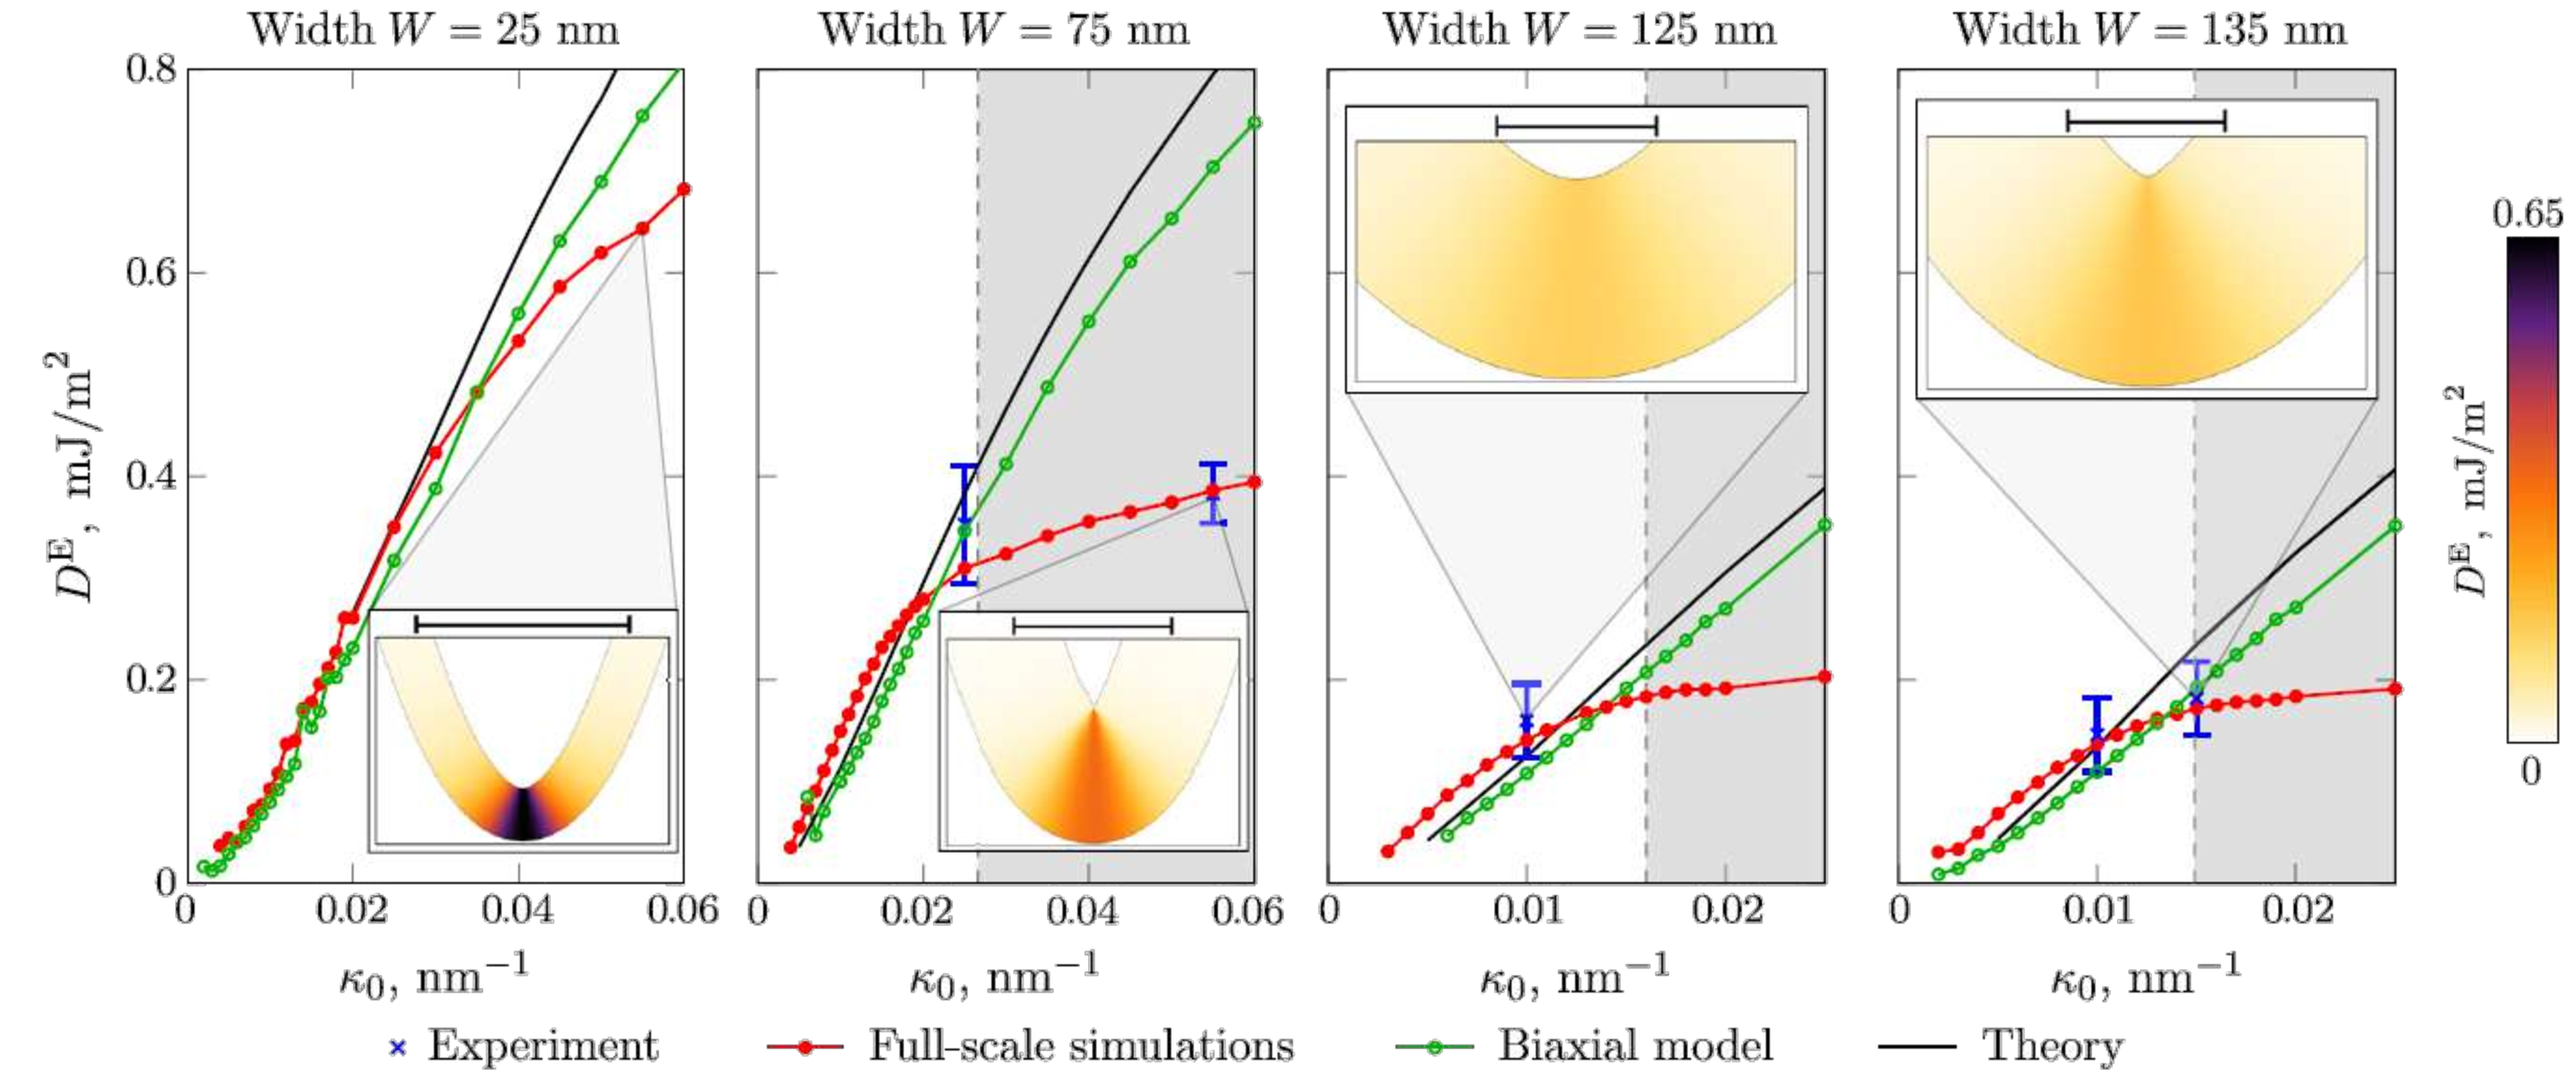
\includegraphics[width=\textwidth]{fig_dmi_parabola}
	\caption{\label{fig:dmi_parabola}%
		\textbf{Geometry-induced DMI constant.} Dependencies of the geometry-induced DMI constants $D^\textsc{e}$ on curvature $\kappa_0$ for different parabolic stripe widths. The inset
			pictures represent the distribution of the $D^\textsc{e}$ along the parabolic stripe apex. Scale bars correspond to 100 nm for all the inset pictures. Figure is reproduced from~\cite{Volkov19c}.}
\end{figure}
%==================================================================/

%The DMI energy density for the curvilinear 1D system reads as~\cite{Volkov18}
%\begin{equation}\label{eq:DMI_FrenetSerret}
%\begin{split}
%\mathcal{E}_\textsc{dm}=\mathcal{E}_\textsc{dm}^0+\mathcal{E}_\textsc{dm}^\textsc{a},\quad \mathcal{E}_\textsc{dm}^0=\mathfrak{D}_{\alpha\beta}\left(m_\alpha \partial_s m_\beta-m_\beta\partial_s m_\alpha\right),\ \quad \mathcal{E}_\textsc{dm}^\textsc{a}=\mathfrak{K}_{\alpha\beta}\,m_\alpha m_\beta,\\
%\mathfrak{D}_{\alpha\beta}=\frac{1}{2}\left(\begin{matrix}
%0 & -D_\textsc{b} & -D_\textsc{n}\\
%D_\textsc{b} & 0 & -D_\textsc{t}\\
%D_\textsc{n} & D_\textsc{t} & 0
%\end{matrix}\right),\quad \mathfrak{K}_{\alpha\beta}=\frac{1}{2}\left(\begin{matrix}
%2\tau D_\textsc{t} & \tau D_\textsc{n} & \kappa D_\textsc{t} + \tau D_\textsc{b}\\
%\tau D_\textsc{n} & 0 & \kappa D_\textsc{n}\\
%\kappa D_\textsc{t} + \tau D_\textsc{b} & \kappa D_\textsc{n} & 2\kappa D_\textsc{b}
%\end{matrix}\right).
%\end{split}
%\end{equation}
%Here, $\vec{D}=\left(D_\textsc{t},D_\textsc{n},D_\textsc{b}\right)$ is a DMI vector with $D_\alpha$ being the curvilinear components. The first term $\mathcal{E}_\textsc{dm}^0$ in \eqref{eq:DMI_FrenetSerret} describes the full set of Lifshitz invariant in the Frenet--Serret reference frame, while the second term $\mathcal{E}_\textsc{dm}^\textsc{a}$ determines the effective geometry-induced anisotropy with anisotropy tensor $\mathfrak{K}_{\alpha\beta}$.

The total energy~\eqref{eq:total_energy} in the curvilinear reference frame reads as
\begin{equation}\label{eq:totalEnergy_FrenetSerret}
\frac{E}{K\mathcal{S}\ell}=\int\limits_{-\infty}^{+\infty}\left[m'_\alpha m'_\alpha+\mathcal{D}_{\alpha\beta}\left(m_\alpha m'_\beta - m'_\alpha m_\beta\right)+\mathcal{K}^{\mu\nu}_{\alpha\beta}m_\alpha m_\beta\right]\mathrm{d}\xi.
\end{equation}
Here, $\mathcal{S}$ is a cross section area, prime denotes to the derivative with respect to the dimensionless coordinate $\xi=s/\ell$, $\mathcal{D}_{\alpha\beta}=\ell\mathcal{F}_{\alpha\beta}$ is the DMI matrix, and $\mathcal{K}^{\mu\nu}_{\alpha\beta}=\ell^2\mathcal{K}_{\alpha\beta}-\delta_{\mu\alpha}\delta_{\mu\beta}+\varepsilon\delta_{\nu\alpha}\delta_{\nu\beta}$ is the anisotropy matrix. One should note that we had not introduce any new interactions in the model \eqref{eq:total_energy} we only present it in the curvilinear reference frame.
%Here, $\mathcal{S}$ is a cross section area, prime denotes to the derivative with respect to the dimensionless coordinate $\xi=s/\ell$. The DMI $\mathcal{D}_{\alpha\beta}=\ell\mathcal{F}_{\alpha\beta}+\mathfrak{D}_{\alpha\beta}/\sqrt{AK}$ and anisotropy $\mathcal{K}^\gamma_{\alpha\beta}=\ell^2\mathcal{K}_{\alpha\beta}+\mathfrak{K}_{\alpha\beta}/\sqrt{AK}-\delta_{\gamma\alpha}\delta_{\gamma\beta}$ matrices are defined as
%\begin{equation}
%\begin{split}
%\mathcal{D}_{\alpha\beta}=&\left(\begin{matrix}
%	0&\varkappa-d_\textsc{b}/2&-d_\textsc{n}/2\\
%	-\varkappa+d_\textsc{b}/2&0&\sigma-d_\textsc{t}/2\\
%	d_\textsc{n}/2&-\sigma+d_\textsc{t}/2&0
%\end{matrix}\right),\\
%\mathcal{K}_{\alpha\beta}^\gamma=&\frac{1}{2}\left(\begin{matrix}
%2\varkappa^2+2\sigma d_\textsc{t}&\sigma d_\textsc{n}&-2\varkappa\sigma+\varkappa d_\textsc{t}+\sigma d_\textsc{b}\\
%\sigma d_\textsc{n}&2\varkappa^2+2\sigma^2&\varkappa d_\textsc{n}\\
%-2\varkappa\sigma+\varkappa d_\textsc{t}+\sigma d_\textsc{b}&\varkappa d_\textsc{n}&2\sigma^2+\varkappa d_\textsc{b}
%\end{matrix}\right)-\delta_{\gamma\alpha}\delta_{\gamma\beta},
%\end{split}
%\end{equation}
%where $\varkappa=\ell \kappa$ and $\sigma=\ell\tau$ are dimensionless curvature and torsion, respectively, and $d_\alpha=D_\alpha/\sqrt{AK}$ is a dimensionless components of DMI vector. One should note that we had not introduce any new interactions in the model \eqref{eq:total_energy} we only present it in the curvilinear reference frame.

\subsection{Equilibrium states in FM curved wires and stripes}\label{sec:statics}

%The developed approach in Refs.~\cite{Sheka15,Volkov18} and described in Sec.~\ref{sec:model_1D} enables us to obtain a general static solution for the high anisotropy case. We consider a physically interesting case of easy-tangential anisotropy, which favours the magnetization distribution tangential to the wire. In the strong anisotropy limit, the magnetization is quasitangential; therefore we expect small deviation of magnetization from tangential direction, i.e. we introduce a small deviation\footnote{We use the following parametrization for the unit magnetization vector $\vec{m}=\sin\theta\cos\phi\,\vec{e}_\textsc{t}+\sin\theta\sin\phi\,\vec{e}_\textsc{n}+\cos\theta\,\vec{e}_\textsc{b}$.} as $\theta=\pi/2+\vartheta$ and $\phi=\phi_0+\varphi$, whereas $|\vartheta|,\ |\varphi|\ll1$ and $\cos\phi_0=\pm1$. Then the total energy density~\eqref{eq:totalEnergy_FrenetSerret} for $\vec{d}=\vec{0}$ can be rewritten as follows $\mathcal{E} \approx \mathcal{E}_\textsc{t}-2\left(\varkappa\varphi'-\cos\phi_0\, \varkappa\sigma\,\vartheta\right)+\left(\vartheta^2+\varphi^2\right)+\text{const}$. Here the first term~$\mathcal{E}_\textsc{t}$ is the energy density of a strictly tangential distribution, the second term is a sum of geometry-induced DMI and anisotropy terms, and the last term determines the anisotropy contribution. Minimization of the energy with respect to $\vartheta$ and $\varphi$ results in equilibrium state

The developed approach in Refs.~\cite{Sheka15,Volkov18} and described in Sec.~\ref{sec:model_1D} enables us to obtain a general static solution for the high anisotropy case. We consider a physically interesting case of easy-tangential anisotropy, which favours the magnetization distribution tangential to the wire. In the strong anisotropy limit, the magnetization is quasitangential; therefore we expect small deviation of magnetization from tangential direction, i.e. we introduce a small deviation\footnote{We use the following parametrization for the unit magnetization vector $\vec{m}=\sin\theta\cos\phi\,\vec{e}_\textsc{t}+\sin\theta\sin\phi\,\vec{e}_\textsc{n}+\cos\theta\,\vec{e}_\textsc{b}$.} as $\theta=\theta_0+\vartheta$ and $\phi=\phi_0+\varphi$, whereas $|\vartheta|,\ |\varphi|\ll1$ and $\cos\phi_0=\pm1$. Then the total energy density~\eqref{eq:totalEnergy_FrenetSerret} for $\tau=0$ and $\varepsilon = 0$ can be rewritten as follows $\mathcal{E} \approx \mathcal{E}_\textsc{t}-2\varkappa\varphi'+\vartheta^2+\varphi^2+\text{const}$ with $\varkappa=\ell\kappa$ being the dimensionless curvature. Here the first term~$\mathcal{E}_\textsc{t}$ is the energy density of a strictly tangential distribution, the second term is a sum of geometry-induced DMI and anisotropy terms, and the last term determines the anisotropy contribution. Minimization of the energy with respect to $\vartheta$ and $\varphi$ results in equilibrium state
\begin{equation}\label{eq:strong_anis_lomit}
%\theta=\frac{\pi}{2}-\varkappa\sigma\cos\phi_0,\quad \phi=\phi_0+\varkappa'.
\theta_0=\frac{\pi}{2},\quad \phi=\phi_0+\varkappa'.
\end{equation}
Solution~\eqref{eq:strong_anis_lomit} shows that magnetization of the equilibrium state always lies within the plane of the wire~(i.e. $\vec{m}\cdot\vec{e}_\textsc{b}=0$), and it is not tangential to the wire if $\varkappa'\neq0$. For the case of ring-shaped wire with $\varkappa=\text{const}$ one obtains a well known \textit{vortex} magnetization distribution~\cite{Klaui03a,Sheka15,Guimaraes17}. This state is typical for relatively large rings~(rings with small curvature) and describes the homogeneous magnetization distribution in the curvilinear reference of frame, see Fig.~\ref{fig:ring_states}. In the opposite case of small rings one obtains a quasi-uniform in Cartesian reference of frame magnetization distribution, see Fig.~\ref{fig:ring_states}. This state is an arrangement of spins in which the ring is divided into two magnetic domains separated by two DW, with magnetizations oriented tangentially in two different directions, clockwise and counterclockwise, a structure that is usually referred to as an \textit{onion} state~\cite{Klaui03a}.

%==================================================================\
\begin{figure}[t]
	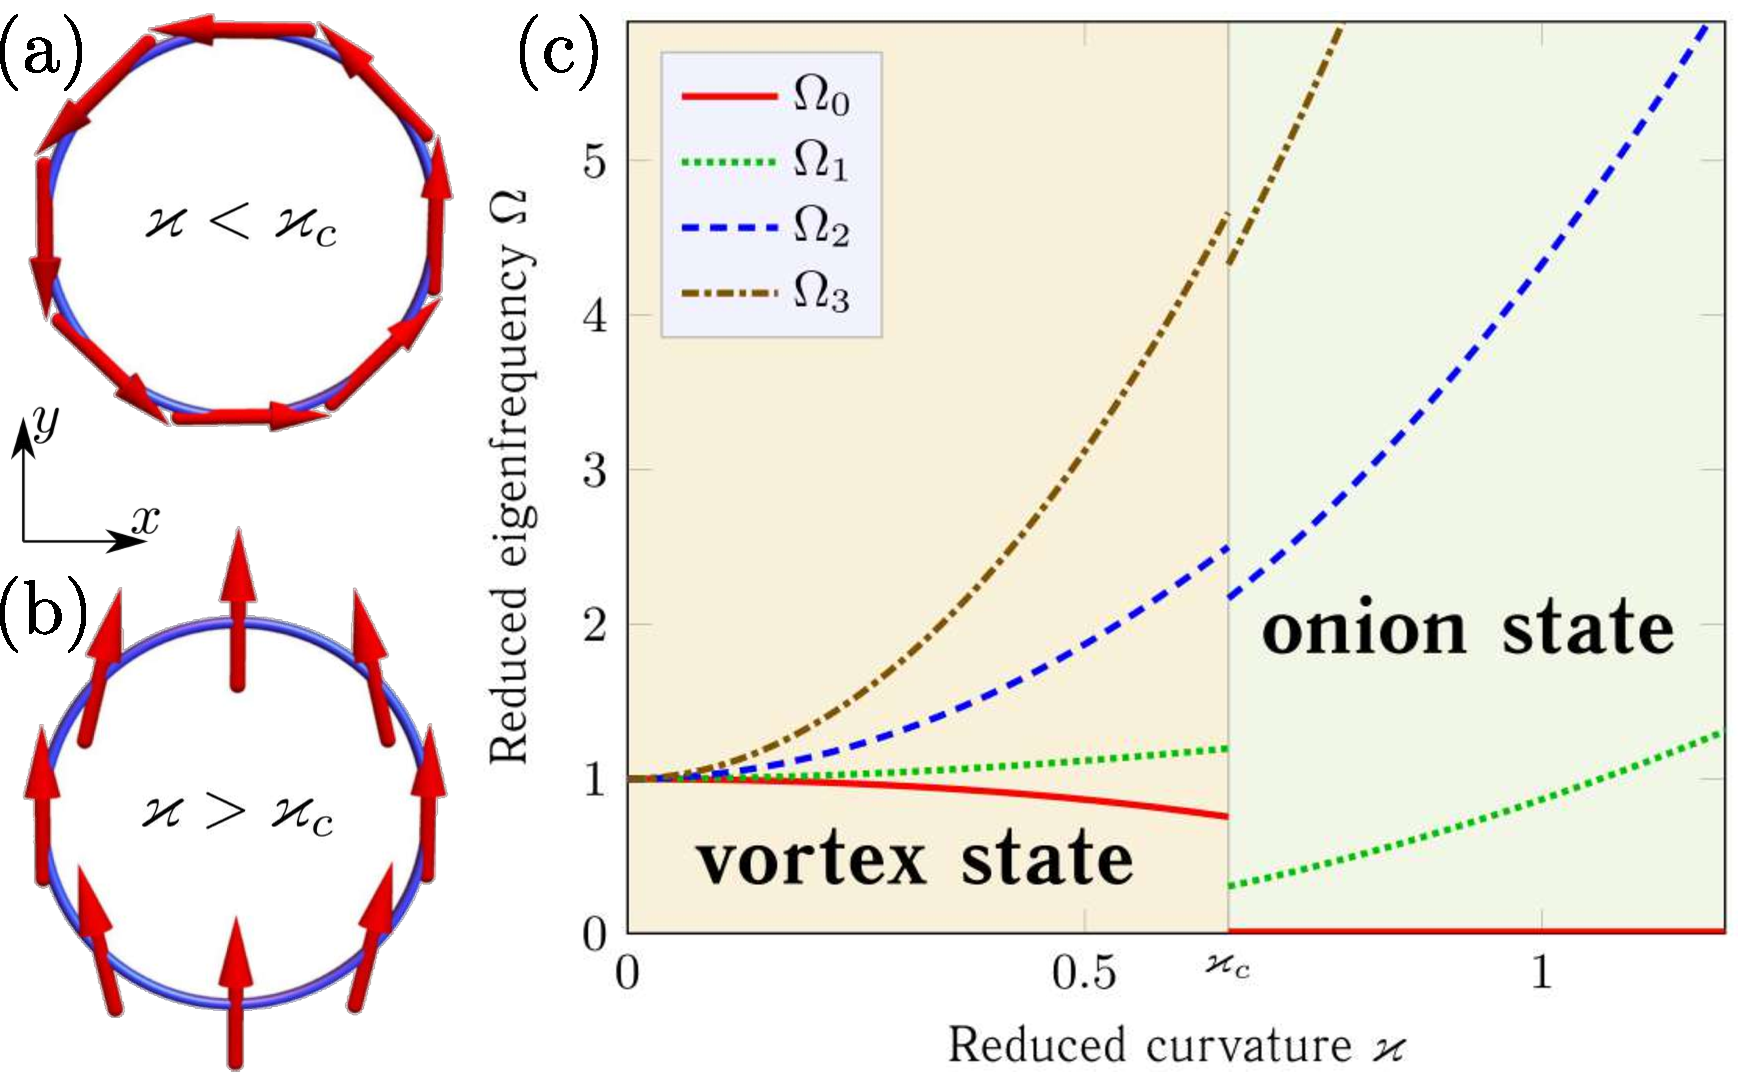
\includegraphics[width=\textwidth]{fig_ring_states}
	\caption{\label{fig:ring_states}%
		\textbf{Equilibrium states in nanorings.} (a) Magnetization distribution of the ground state in a ring wire with different reduced curvatures: vortex state for $\varkappa<\varkappa_c$ and onion state for $\varkappa>\varkappa_c$. (b) Hysteresis curve of polycrystalline  Co nanorings array exhibiting vortex and onion states. Red arrows indicate the field path used to obtain the rings in the states imaged with PEEM in (c). (c) A PEEM image of	four polycrystalline Co rings. (d) Spin structure of (d$^1$) a vortex wall and (d$^2$) a transverse wall simulated using the OOMMF code. PEEM images of (d$^3$) a 30 nm thick and 530 nm wide, (d$^4$) a 10 nm thick and 260 nm wide, and	(d$^5$) a 3 nm thick and 730 nm wide ring. The gray scale shows	the magnetization direction. Panel (a) is reproduced from~\cite{Sheka15}; (b) and (c) are reproduced from~\cite{Klaui03a}; (d) is reproduced from~\cite{Laufenberg06}.}
\end{figure}
%==================================================================/

Nanorings with \textit{vortex} magnetization ground state can be prepared with smaller radii than nanodisks with the same spin structure~\cite{Kravchuk07}. This nanoring critical radius which separates the \textit{vortex} and \textit{onion} states defined, in general, by the relation~\cite{Sheka15}:
\begin{equation}\notag
R_{c} = \varkappa_c^{-1}\sqrt{A/K},\quad \varkappa_c \approx 0.657.
\end{equation}
For the permalloy nanoring we have $R_{c}\approx 17$ nm, i.e. for rings with $R>R_c$ one obtains \textit{vortex} state, while for $R<R_c$ -- \textit{onion} state.

As it was mentioned above that two domains in the \textit{onion} state are separated by two DWs. Depending on the width of the ring one can obtain a transverse head-to-head~(tail-to-tail) DWs for narrow ribbons, or vortex head-to-head~(tail-to-tail) DWs for wide rings, see Fig.~\ref{fig:ring_states}.

%==================================================================\
\begin{figure}[t]
	\includegraphics[width=\textwidth]{fig_cornu_n_meander}
	\caption{\label{fig:cornu_n_meander}%
		\textbf{Equilibrium states in curved wires.} (a) and (c) Spatial distribution of magnetization (red arrows) along the wires with the shape of meander and Euler spiral; the inclination angle $\phi$ is shown in insets. (b) Inclination angle $\phi$ as function of arc length for meander shaped wire with $\varkappa_0=0.6$: line -- analytical solution, dots -- results of numerical simulations. Panels (a) and (b) are reproduced from~\cite{Korniienko19b}.}
\end{figure}
%==================================================================/

The deviation of magnetization from  strictly tangential direction in circle segment with $\varkappa<\varkappa_c$ can be observed in wires with periodically repeated semicircles of curvature $\varkappa_0$~\cite{Korniienko19b}, see Fig.~\ref{fig:cornu_n_meander}(a). The spatial distribution of the curvature of such a wire is the square-wave function $\varkappa(\xi) = (-1)^{\lfloor\xi/\xi_0\rfloor}\varkappa_0$ with period $2\xi_0$, $\xi_0=\pi/\varkappa_0$, and $\lfloor x \rfloor$ defines the integer part of $x$. The corresponding inclination $\phi$ for square-wave function $\varkappa(\xi)$ reads~\cite{Korniienko19b}
\begin{equation}\label{eq:phi_meander}
\phi = (-1)^\lambda \text{am}\left[\frac{\xi-\xi_0\left(\lambda+1/2\right)}{k},ik\right],\quad \lambda=\lfloor \xi/\xi_0 \rfloor,\quad k=\frac{1}{\sqrt{\varkappa_0^2-\sin^2\varphi_0}},
\end{equation}
where $\text{am}\left(x,y\right)$ is Jacobi amplitude~\cite{NIST10}. Constant $\varphi_0=|\phi\left(n\xi_0\right)|$ is maximal value of the function $\phi(\xi)$ [see Fig.~\ref{fig:cornu_n_meander}(b)], it is determined by the equation $2kF(\varphi_0,ik) = \xi_0$, where $F(x,y)$ is elliptic integral of the first kind~\cite{NIST10} and the modulus $k = k(\varphi_0)$ is defined in~\eqref{eq:phi_meander}. One should note that the curvature amplitude $\varkappa_0$ is the only parameter which controls the system. The maximal deviation $\varphi_0$ from the tangential direction takes place in points of junction of two semicircles, this is because of the curvature jump. Depending on the $\varkappa_0$ one obtains two different behaviors~\cite{Korniienko19b}: (i) In the limit case of small curvature $\varkappa_0\ll1$ and due to the easy-tangential anisotropy the wire is magnetized practically tangentially except the junction points, where the magnetization demonstrates the small deviations of amplitude $\varphi_0\approx\varkappa_0$. (ii) In the opposite case of large curvature $\varkappa_0\gg1$ exchange interaction is dominating and results in quasi uniform magnetization aligned with $x$-axis with $\varphi_0\lesssim\pi/2$.

For the specific case of the wire with constant gradient of the curvature $\varkappa'=\chi=\text{const}$ [wire with a shape of Euler spiral~\cite{Lawrence14}, also known as Cornu spiral or clothoid, see Fig.~\ref{fig:cornu_n_meander}(c)], geometry-induced magnetization inclination from the tangential direction can be calculated analytically~\cite{Yershov18a}. One can find that magnetization deviates from the tangential direction as $\phi=\phi_0+\arcsin(2\chi)/2$~\cite{Yershov18a}, also see Fig.~\ref{fig:cornu_n_meander}(c). This solution coincides with~\eqref{eq:strong_anis_lomit} for the limit case of small gradient of the curvature $\chi\ll1$.

Similar geometry-induced inclination of magnetization from anisotropy axis were also obtained for wires with box-function curvature~\cite{Gaididei18a}.


\subsection{Linear dynamics in FM curved flat wires and stripes}\label{sec:linear_dyn}

%	In this section we can discuss the spin-wave dynamics in curved systems:
%	\begin{itemize}
%		\item magnon spectrum in the ring~\cite{Sheka15}
%		\item local modes \& magnon filter ~\cite{Gaididei18a,Korniienko19b}
%	\end{itemize}

Approach described in Sec.~\ref{sec:model_1D} allows also to study the linear dynamics of magnons on the background of equilibrium states. To analyse the magnons in the curved system, we linearize the Landau--Lifshitz--Gilbert equation~\eqref{eq:llg} for zero damping $\alpha_\textsc{g}=0$ on the background of the equilibrium state~\eqref{eq:strong_anis_lomit} with the substitution $\theta=\theta_0+\vartheta(t,\xi)$ and $\phi=\phi_0+\varphi(t,\xi)$. The linearizaed equations of motion reads as~\cite{Sheka15,Gaididei18a,Korniienko19b}
\begin{equation}\label{eq:linear_magnons}
    -\vartheta''&+V_1\vartheta = \dot{\varphi},\quad  -\varphi''&-V_2\varphi = -\dot{\vartheta},
\end{equation}
where $V_1 = \cos^2\phi - \left[\phi'+\varkappa(\xi)\right]^2$ and $V_2 = \cos2\phi$ are geometry-induced potentials, and overdot indicates the dirivative with respect to reduced time $\overline{t}=t\gamma_0K/M_s$. For the simplest case of the ring-shaped wire with constant curvature $\varkappa=\text{const}$ one obtain $V_1=1-\varkappa^2$ and $V_2=1$. The set~\eqref{eq:linear_magnons} for the case of the ring wire with periodic boundary conditions can be solved with plane waves ansatz $\vartheta=\sum_j \vartheta_j \cos(j\xi\varkappa-\Omega\overline{t}+\delta_j)$ and $\varphi=\sum_j \varphi_j \sin(j\xi\varkappa-\Omega\overline{t}+\delta_j)$ with $j$ being the azimuthal quantum number, $\delta_j$ is an arbitrary phase, and $\Omega$ is dimensionless frequency measured in units $\gamma_0K/M_s$. By substituting this ansatz in the set~\eqref{eq:linear_magnons} we can calculate the spectrum of magnon eigenstates as
\begin{equation}\label{eq:spec_rings}
    \Omega^\text{ring}_j = \sqrt{\left(1+j^2\varkappa^2\right)\left(1+j^2\varkappa^2 - \varkappa^2\right)}.
\end{equation}
For the limit case of the small curvature $\varkappa\ll1$~(quasi-straight wire), the magnon frequencies read
\begin{equation}\label{eq:spec_rings_small}
    \Omega^\text{ring}_j = 1- \frac{\varkappa^2}{2}+j^2\varkappa^2+\mathcal{O}(\varkappa^4).
\end{equation}
Thus the curvature decreases the gap as compared to the case of the straight wire~($\varkappa=0$) with dispersion $\Omega^\text{str} = 1 + \mathfrak{K}^2$, where $\mathfrak{K}=j\varkappa$ is the corresponding normalized wave vector.

One can combine the set of Eq.~\eqref{eq:linear_magnons} in a single equation for a complex valued function $\psi=\vartheta+i\varphi$, which has the form of the generalized Schr\"odinger equation
\begin{equation}
    \begin{split}
       -i\dot{\psi} = \mathcal{H}\psi+\mathcal{W}\psi^*,& \quad \mathcal{H}=-\partial_\xi^2+\mathcal{U},\\
       \mathcal{U} = \frac{V_1+V_2}{2},\quad &\mathcal{W} = \frac{V_1-V_2}{2}.
    \end{split}
\end{equation}
The form and structure of potentials $\mathcal{U}$ and $\mathcal{W}$ are defined by the curvature and its gradients~\cite{Gaididei18a,Korniienko19b}. 

\subsection{Domain walls in FM curved flat wires and stripes}\label{sec:DW_dyn}

Novel concepts for magnetic logic~\cite{Allwood05} and storage~\cite{Parkin08} devices rely on DW motion inside curvilinear segments, e.g. U-shaped segments in the magnetic racetrack memory~\cite{Parkin08}. Therefore, the modification of dynamic and static properties of a DW due to the wire curvature is of high importance for the applications.

\subsubsection*{Statics of DW.} Collective variable approach is widely used to analyze properties of soliton-like excitations. We use a collective variable approach based on the $q-\Phi$ model~\cite{Slonczewski72,Malozemoff79}
\begin{equation}\label{eq:q_phi_model}
\cos\theta=-p\tanh\left[\frac{\xi-q(t)}{\Delta}\right],\quad\phi=\Phi(t),
\end{equation}
where $\{q, \Phi\}$ are time-dependent conjugated collective variables, which determine the DW position and orientation of transverse magnetization component, respectively; $\Delta$ is a DW width; $p$ is a topological charge, which determines the DW type: head-to-head ($p = +1$) or tail-to-tail ($p = -1$). Here $q$ and $\Delta$ are dimensionless quantities measured in the units of magnetic length $\ell$. The Ansatz~\eqref{eq:q_phi_model} coincides with the exact DW solution for a rectilinear wire ($\varkappa=0$ and $\vec{d}=\vec{0}$). Here, the curvature is considered as a small perturbation, which keeping the form~\eqref{eq:q_phi_model} unchanged. The DW width $\Delta$ is shown to be a slaved variable~\cite{Hillebrands06} even in the flat curvilinear systems~\cite{Yershov18a}, i.e. $\Delta(t) = \Delta\left[q(t),\Phi(t)\right]$.

The energy~\eqref{eq:totalEnergy_FrenetSerret} for DW reads
\begin{equation}\label{eq:dw_energy}
	\frac{E^\textsc{dw}}{2K\mathcal{S}\ell}\approx\frac{1}{\Delta}+\Delta\,\left(1+\varepsilon\sin^2\Phi\right)+p\pi\varkappa(q)\cos\Phi+\mathcal{O}\left(\varkappa^2\right),
\end{equation}
where the condition $\varkappa\Delta\ll1$ was applied when integrating. Similar expression were obtained for the DW energy in the circular wire segment~\cite{Kruger07a}. The first and second terms represent the competition between the isotropic exchange and anisotropy terms, and defines the DW width in rectilinear system. While the last terms determine the geometry-induced DMI and anisotropy terms, respectively.

Firstly, lest us consider the systems with localized curvature $\varkappa(\pm\infty)=0$, i.e. parabola-shaped system. Minimization of~\eqref{eq:dw_energy} with respect to $q$ and $\Phi$ results in the following equilibrium values
\begin{equation}\label{eq:dw_eq_state}
\varkappa'\left(q_0\right)=0,\quad\cos\Phi_0=-p.
\end{equation}
The first equation in~\eqref{eq:dw_eq_state} corresponds to DW pinning at the maximum of the curvature. While, the second equation demonstrates process of a symmetry breaking due to the geometry-induced DMI~\cite{Yershov15b}: transverse magnetization of a head-to-head (tail-to-tail) DW is directed outwards (inwards), see Fig.~\ref{fig:dw_wire_1}(a). The latter effect was recently observed experimentally~\cite{Kim14,Volkov19c}, see Figs.~\ref{fig:dw_wire_1}(b),~\ref{fig:dw_wire_1}(d),~\ref{fig:dw_wire_1}(e). There is an intuitive explanation: the choice of $\Phi_0$ defined by~\eqref{eq:dw_eq_state} makes the magnetization distribution more homogeneous, see Figs.~\ref{fig:dw_wire_1}(a) and~\ref{fig:dw_wire_1}(b), which decreases energy of the geometry-induced DMI term in~\eqref{eq:dw_energy}. One should note that such a phase selectivity for DWs also takes place in the systems with constant curvature~\cite{Moreno17a} and in rings in the onion state, see Figs.~\ref{fig:ring_states}(a) and \ref{fig:ring_states}(d$^2$). It should be noted that circular geometry does not produce any geometrical pinning potential due to the constant curvature $\varkappa=\text{const}$, which results in undefined $q_0$. Nevertheless, the domain wall can have an equilibrium position in circular segment in the presence of an external magnetic field~\cite{Kruger07a,Jamali11}.

%==================================================================\
\begin{figure}[t]
	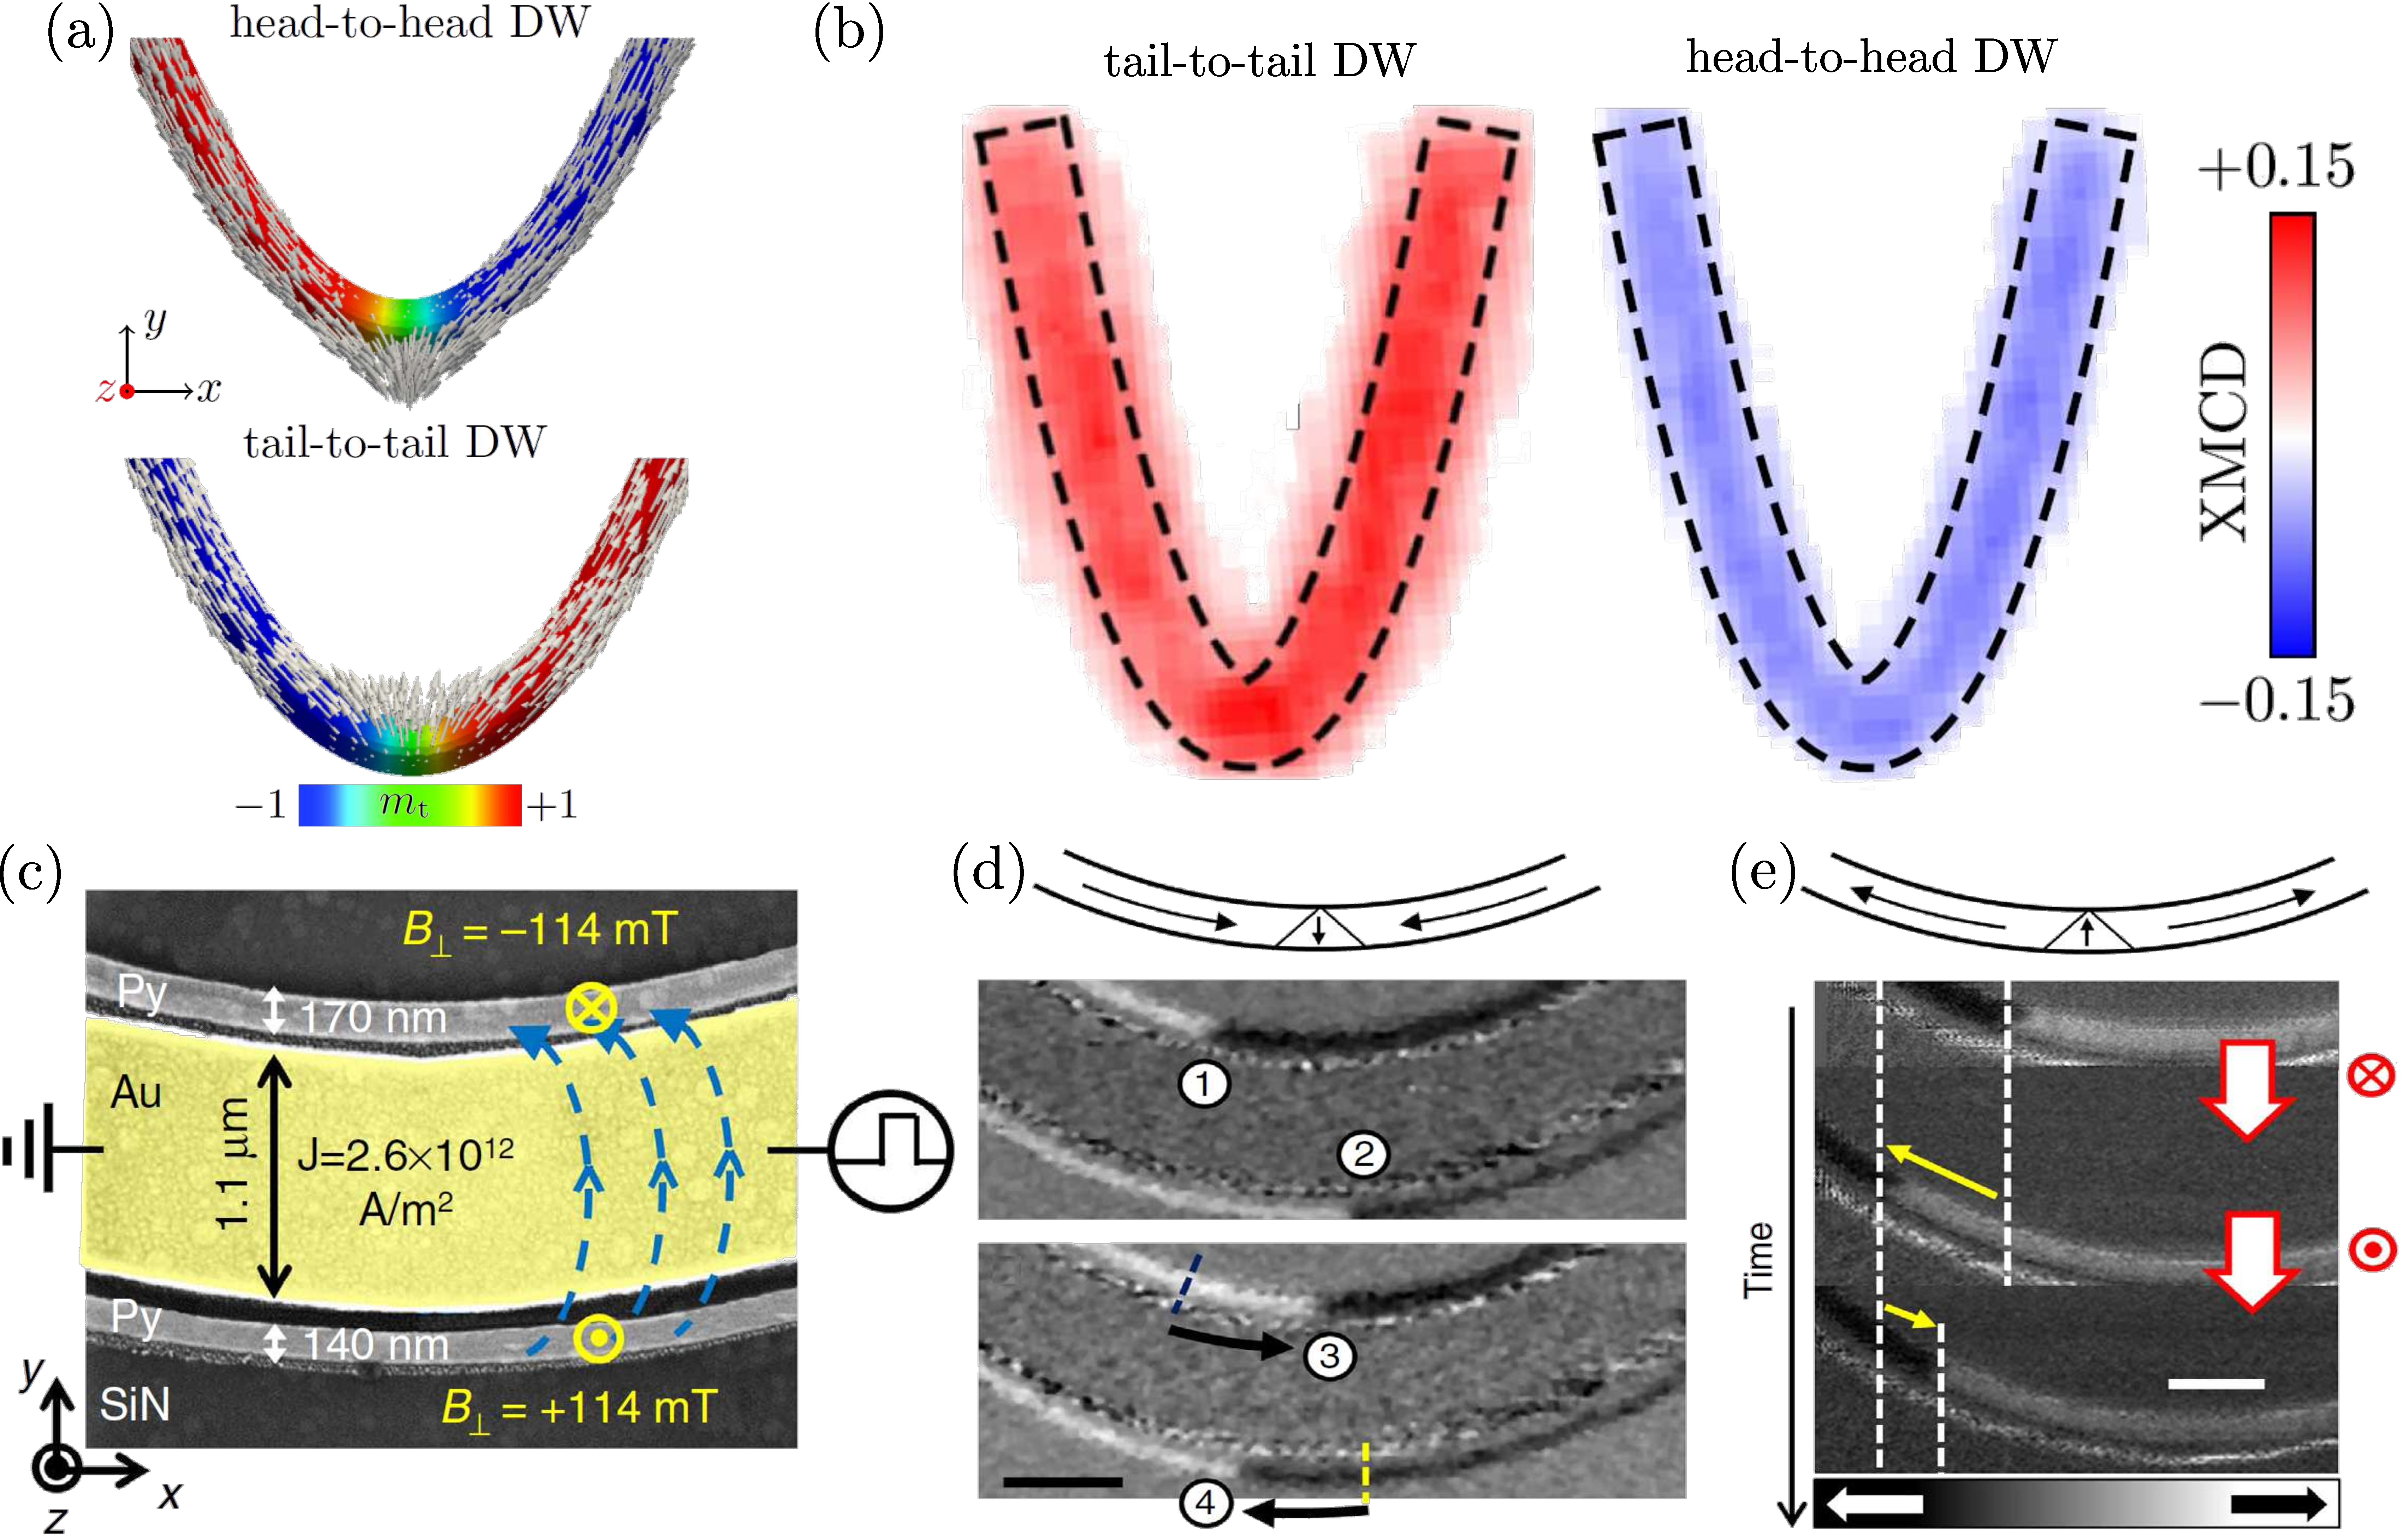
\includegraphics[width=\textwidth]{fig_dw_curved_wire}
	\caption{\label{fig:dw_wire_1}%
		\textbf{DW in a flat wire bend.} (a) Equilibrium state of the transverse DW at the wire bend obtained by means of micromagnetic simulations. (b) Magnetic states imaged by XMCD-PEEM of tail-to-tail and head-to-head DWs. (c) Scanning electron microscopy image of two curved planar nanowires embedding a strip line (yellow shaded), which generates out-of-plane magnetic	fields with opposite direction at each nanowire. (b) and (c) show the scanning transmission x-ray microscopy images visualizing DWs. (d) Initial and final displacement of DWs after five subsequent field pulses as indicated in (a). In (d) the upper DW moves a distance of $840\pm20$nm from position (1) to position (3), while the lower DW travels $940\pm20$nm from position (2) to position (4). Scale bar, 1 mm. (e) Same for upper nanowire and opposite current pulses. DW travels ($680 \pm 20$) nm to the left and ($340\pm20$) nm to the right, respectively. Scale bar: 500 nm. Panel (a) is reproduced from~\cite{Yershov15b}; panel (b) is reproduced from~\cite{Volkov19c}; panels (c), (d), and (e) are reproduced from~\cite{Kim14}.}
\end{figure}
%==================================================================/

\subsubsection*{Dynamics of DW.} The dynamics of magnetization is governed by the phenomenological Landau--Lifshitz--Gilbert equation~\eqref{eq:llg}. In terms of $\{q,\Phi,\Delta\}$ it reads~\cite{Yershov15b,Yershov18a}
\begin{equation}\label{eq:dw_qPhi_motion}
\begin{split}
\frac{\alpha}{\Delta}\dot{q}+p\dot{\Phi} = &-p\pi\frac{\partial\varkappa(q)}{\partial q}\cos\Phi,\\
p\dot{q}-\alpha\Delta\dot{\Phi} = &-p\pi\varkappa(q)\sin\Phi+\varepsilon\Delta\sin 2\Phi,
\end{split}
\end{equation}
where $\alpha$ is a Gilbert damping parameter, overdot correspond to the derivative with respect to dimensionless time $\overline{t}=t\gamma_0K/M_s$ with $\gamma_0$ being the gyromagnetic ratio and $M_s$ saturation magnetization.
The dynamics of the DW width can be described as $\alpha\pi^2\dot{\Delta}/12=1/\Delta-\Delta\left(1+\varepsilon\sin^2\Phi\right)$, which shows that $\Delta$ relaxes towards its equilibrium value $\Delta_0=1/\sqrt{1+\varepsilon\sin^2\Phi}$. The characteristic time of this relaxation is proportional to the damping $\propto \alpha$~\cite{Hillebrands06}. Usually $\alpha\ll1$, therefore one can conclude that the DW width is a slave variable $\Delta(t) = \Delta[\Phi(t)]$ and DW dynamics can be described by the set~\eqref{eq:dw_qPhi_motion}  with the equilibrium DW width $\Delta=\Delta_0$. From \eqref{eq:dw_qPhi_motion} it follows that the gradient of the curvature is a driving force for DWs. The physical origin of this force is the geometry-induced DMI driven by the exchange.

%==================================================================\
\begin{figure}[t]
	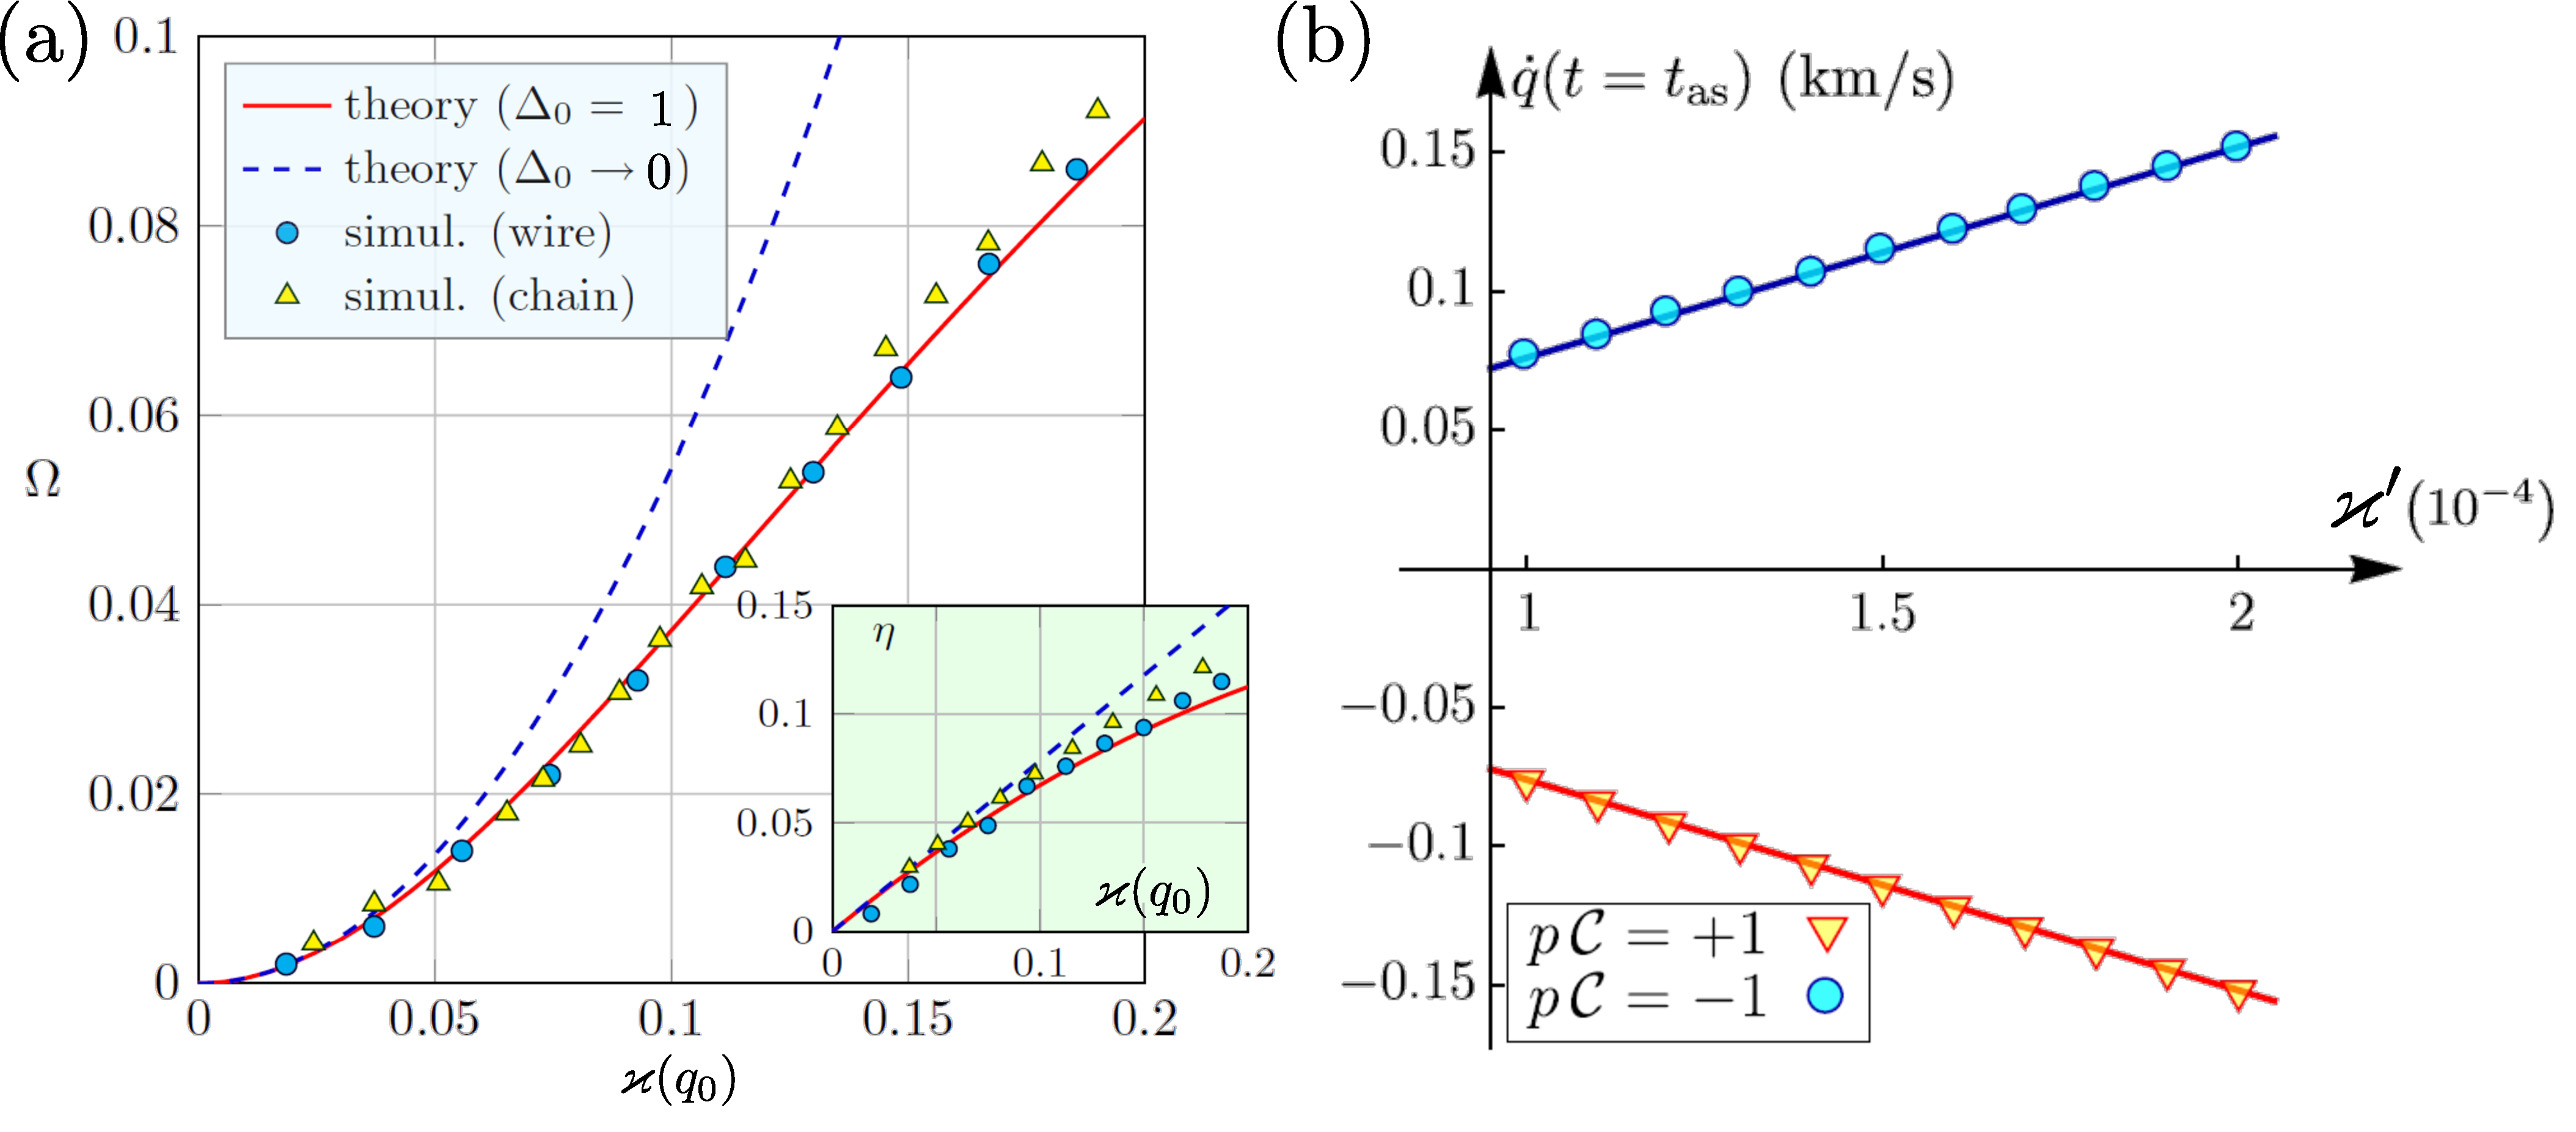
\includegraphics[width=\textwidth]{fig_dw_dynamics_curved}
	\caption{\label{fig:dw_wire_2}%
		\textbf{DW dynamics in curved wires.} (a) Eigenfrequency of the DW oscillations in vicinity of the equilibrium -- the extreme point of parabolic wire bend. (b) DW velocity $\dot{q}$ as a function of the gradient of the curvature in the Euler spiral. In (a) and (b)  lines correspond to the analytical predictions and symbols to the results of micromagnetic simulations. Panel (a) is reproduced from~\cite{Yershov15b}; panel (b) is reproduced from~\cite{Yershov18a}.}
\end{figure}
%==================================================================/

The equations of motion~\eqref{eq:dw_qPhi_motion} can be linearized with respect of small deviations of DW position $\tilde{q}=q-q_0$ and phase $\tilde{\phi}=\Phi-\Phi_0$ in the vicinity of equilibrium position~\eqref{eq:dw_eq_state}. For the limit case of small curvature $\varkappa\ll1$ and $\varepsilon=0$ the equations of motion~\eqref{eq:dw_qPhi_motion} linearized with respect to the deviations reads~\cite{Yershov15b}
\begin{equation}\label{eq:dw_qPhi_motion_linear}
\left(1+\alpha^2\right)\left\|\begin{matrix}
\dot{\tilde{q}}\\
\dot{\tilde{\phi}}
\end{matrix}\right\|=\pi\left\|\begin{matrix}
0 & \varkappa(q_0)\\
\varkappa''(q_0)&-\alpha\varkappa(q_0)
\end{matrix}\right\|\cdot\left\|\begin{matrix}
\tilde{q}\\
\tilde{\phi}
\end{matrix}\right\|.
\end{equation}
For the case of small damping the solution of~\eqref{eq:dw_qPhi_motion_linear} results in harmonic decaying oscillations, see Fig.~\ref{fig:dw_wire_1}(d), with frequency $\Omega$ and modified effective friction $\eta$ defined as
\begin{equation}
\Omega \approx \pi\sqrt{|\varkappa(q_0)\varkappa''(q_0)|},\quad \eta\approx \alpha\frac{\pi}{2}\varkappa(q_0).
\end{equation}
Eigenfrequency of the DW oscillations in vicinity of the equilibrium position is presented in Fig.~\ref{fig:dw_wire_2}(a). As it was mentioned above, the circular geometry does not generate any pinning potential, therefore the eigenfrequency of the DW oscillations in such geometry is $\Omega=0$. The value of pinning potential increases with the increasing of the curvature, see Fig.~\ref{fig:dw_wire_2}(a), which results in the increasing of the deppining field up to 60-80 mT~\cite{Volkov19c,Lewis09}.

Remarkably, that for the wires with monotonic increasing/decreasing curvature as a function of the arc length the curvature gradient in Eqs.~\eqref{eq:dw_qPhi_motion} results in a driving force, i.e. DW can be moved without any external driving~(field or current) and pinning. In the limit case of Euler spiral the DW can move with constant velocity
\begin{equation}\label{eq:velocity_euler_spiral}
V=-p\,\mathcal{C}\,\frac{\varkappa'}{\alpha},\quad\cos\Phi_0=\mathcal{C}=\pm1.
\end{equation}
The phase during the dynamics behaves as $\Phi\approx\Phi_0+p/\left(\alpha V \overline{t}\right)$, which in long time approximation results in $\Phi\left(\overline{t}\to\infty\right)=\Phi_0$. Hence, the parameter $\mathcal{C}$ is interpreted as the DW magnetochirality~\cite{Kim14}.  The corresponding geometry-induced DW velocity for the Euler spiral reaches up to 150 m/s, see Fig.~\ref{fig:dw_wire_2}(b). For the case of curved wires~\cite{Lewis09,Nahrwold09,Wartelle18} with curvature in the range $\kappa\in\left[0;1/150\right]$ nm$^{-1}$ the corresponding curvature-induced DW velocity is expected to be about 80 m/s.

The direction of the geometry-induced DW motion\footnote{One has to notice a one-to-one correspondence between natural	parameter $\xi$ and gradient of the curvature $\varkappa'$ with DW magnitochirality $\mathcal{C}$: change of the natural parameter sign results in the changing of gradient of the curvature and DW magnitochirality	signs, therefore direction of DW motion physically is the same.} is determined by the product of the DW magnetochirality, topological charge, and gradient of the curvature $V\propto p\,\mathcal{C}\varkappa'$, see Fig.~\ref{fig:dw_wire_2}(b). The geometry-induced dynamics are accompanied by the DW motion in the area of bigger curvature. In this way, in the energy~\eqref{eq:dw_energy} the geometry-induced DMI term becomes dominant. This term fixes the DW phase $\cos\Phi=\pm1$, which depends on the sign of the product of the topological charge $p$ and curvature $\varkappa$, see Eq.~\eqref{eq:dw_energy}. Therefore, the transition to the precessional regime becomes suppressed. This effect can be interpreted as the curvature-induced suppression of the Walker limit~\cite{Yershov18a}. This is in contrast to the case of field-driven DWs in a straight wire, where the phase of the DW is not fixed (Zeeman term in the energy of DW is independent of the phase~\cite{Malozemoff79,Hillebrands06}).

One can see that DW velocity is increasing with decreasing Gilbert damping~$\alpha$, see Eq.~\eqref{eq:velocity_euler_spiral}. For the limit case of vanishing damping~($\alpha\to0$) the velocity of the DW increases exponentially with time, and its transverse magnetization component orients perpendicular to the wires plane with $\Phi(\alpha=0)\to-\mathcal{C}\pi/2$.

The DW velocity~\eqref{eq:velocity_euler_spiral} is similar to the well-known expression $V_u = u \beta/\alpha$ in magnetic stripes with biaxial anisotropy caused by the Zhang--Li mechanism~\cite{Bazaliy98,Zhang04}, where $\beta$ is a nonadiabatic spin-transfer parameter. Current-induced translational DW motion takes place only if $u<u_\textsc{w}$, where $u_\textsc{w}$ is Walker current~\cite{Thiaville05}. However, for the case of a geometry-induced motion, a Walker-limit-like effect of the transition to the precessional regime does not appear and the DW demonstrates a high-speed translational motion without any external driving. However, for the current-induced dynamics of DW in an uniaxial~($\varepsilon=0$) circular-shaped wires~($\varkappa=\text{const}$) curvature results in the appearance of Walker limit~\cite{Yershov16}
\begin{equation}
u_\textsc{w}^\varkappa=\frac{\alpha}{|\alpha-\beta|}\pi\varkappa.
\end{equation}

%Geometry-induced motion of DWs desctibed by Eqs.~\eqref{eq:dw_qPhi_motion} can be compared with so called automotion of DW in curved systems~\cite{Chauleau10,Richter16,Mawass17}. This type of motion can be realized relying on: (i) The transformation of DWs from transverse to vortex types after the action of current pulse~\cite{Chauleau10}, see Figs.~\ref{fig:automotion}(a)-\ref{fig:automotion}(f). In this case, the motion of DW is caused by the modification DW phase $\Phi$~(a canonically conjugated variable to DW position $q$). Such type of motion is possible for the duration of excitation is short compared to the relaxation time of the DW structure~\cite{Chauleau10}. (ii) The second mechanism is relying on the motion of DWs in systems with coordinate-dependent cross sectional area of a nanostripe~\cite{Richter16,Mawass17}, see Fig.~\ref{fig:automotion}(g). In this case, the motion of DW is caused by the minimization of DW energy in the narrow area of asymmetric ring~\cite{Mawass17}. One should note that with increasing the gradient of ring's aspect ratio the velocity of DW increases.

Geometry-induced motion of DWs desctibed by Eqs.~\eqref{eq:dw_qPhi_motion} can be compared with so called automotion of DW in curved systems~\cite{Chauleau10,Richter16,Mawass17}. This type of motion can be realized relying on: (i) The transformation of DWs from transverse to vortex types after the action of current pulse~\cite{Chauleau10}. In this case, the motion of DW is caused by the modification DW phase $\Phi$~(a canonically conjugated variable to DW position $q$). Such type of motion is possible for the duration of excitation is short compared to the relaxation time of the DW structure~\cite{Chauleau10}. (ii) The second mechanism is relying on the motion of DWs in systems with coordinate-dependent cross sectional area of a nanostripe~\cite{Richter16,Mawass17}. In this case, the motion of DW is caused by the minimization of DW energy in the narrow area of asymmetric ring~\cite{Mawass17}. One should note that with increasing the gradient of ring's aspect ratio the velocity of DW increases.

%==================================================================\
%\begin{figure}[t]
%	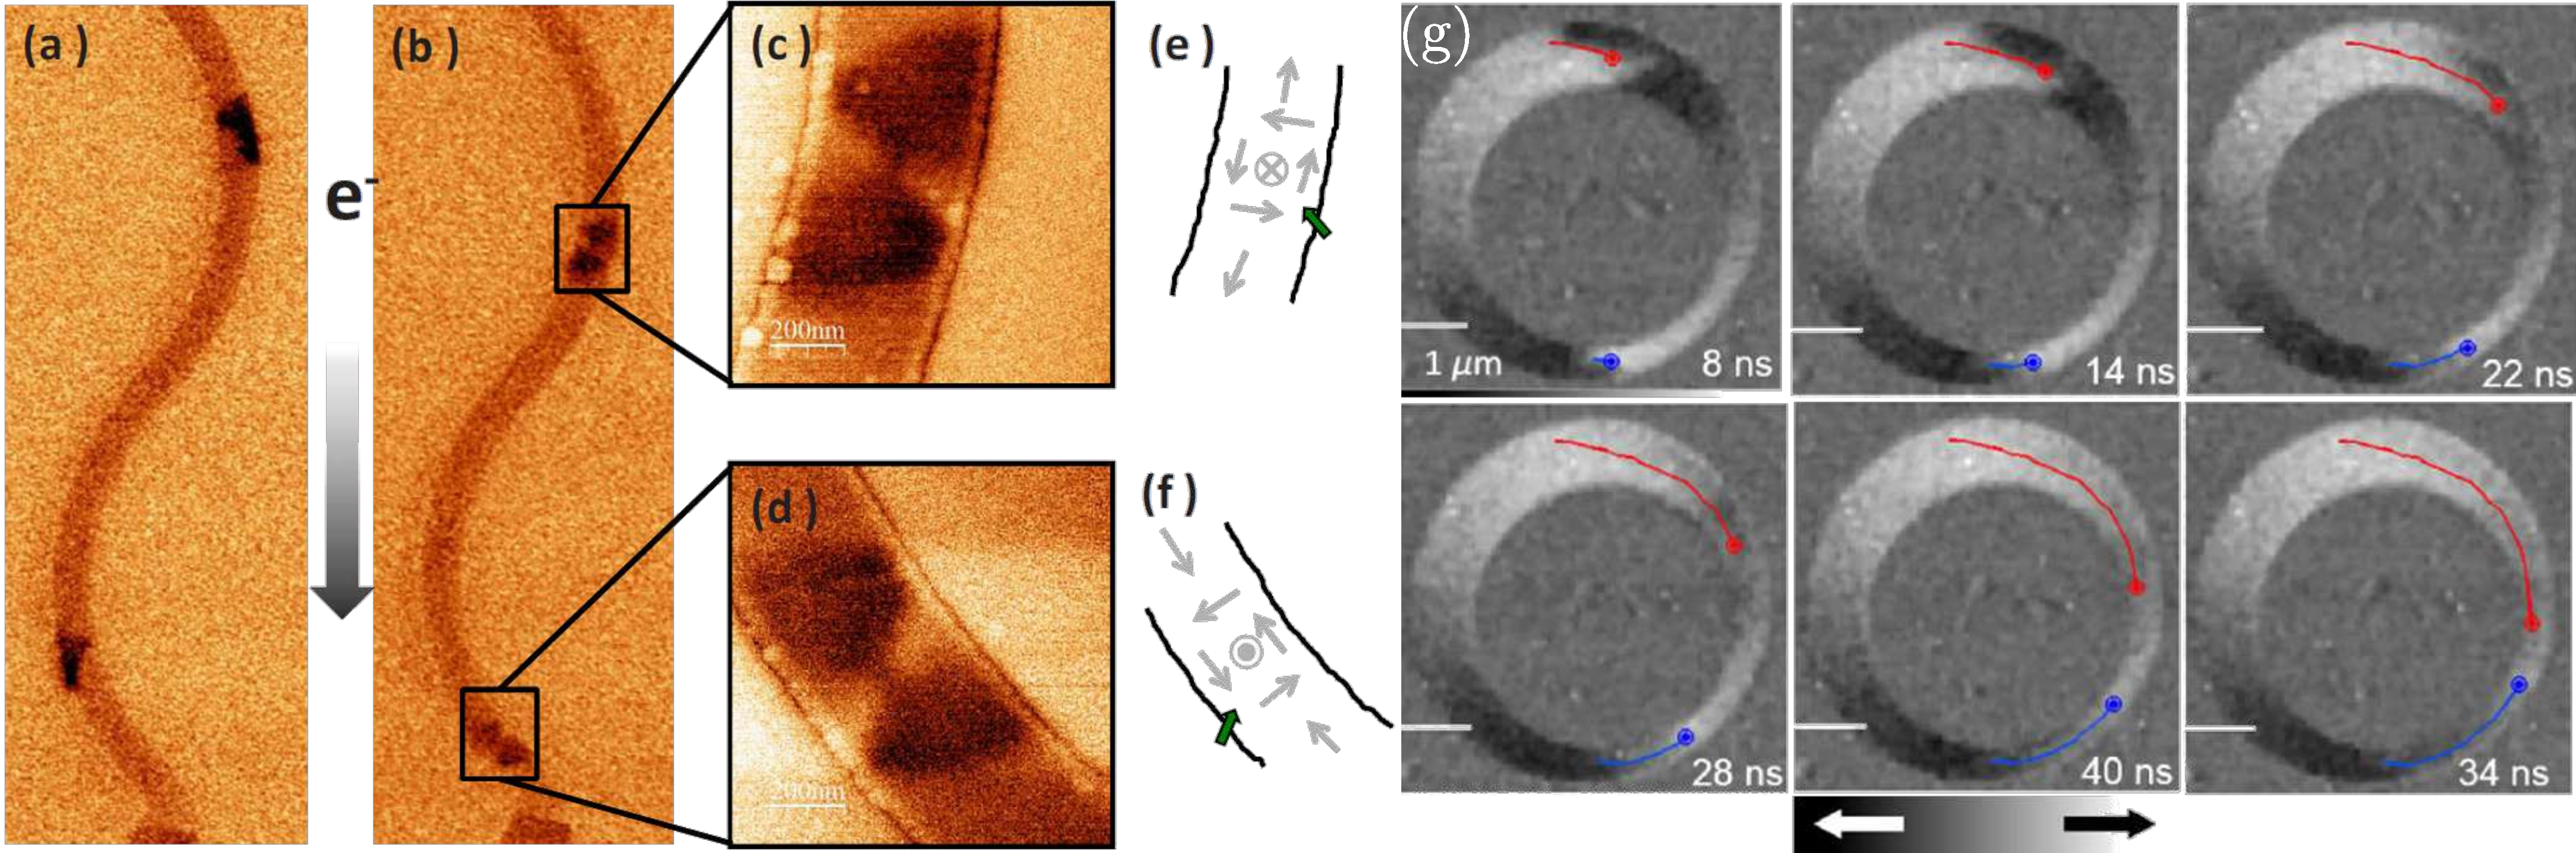
\includegraphics[width=\textwidth]{fig_automotion}
%	\caption{\label{fig:automotion}%
%		\textbf{Automotion of DWs.} (a)-(b) Magnetic force microscopy images of the initial and final magnetic states of the entire S-shaped nanostrip showing two transverse and two vortex DWs, respectivelly . In (b) two vortex DWs displaced by 1.5 and 1.7 $\mu$m after transforming under a 1 ns current pulse of 3.6 TA/m$^2$ amplitude. (c) and (d) zoom on the vortex DWs, with schematics shown in (e) and (f). (g) Time-resolved STXM XMCD snapshots of automotive DWs motion during the switching process from the onion to the vortex state in the ferromagnetic ring. Red and blue lines in (g) illustrate the averaged trajectory of the vortex DWs. Panels (a)-(f) are reproduced from~\cite{Chauleau10}; panel (g) is reproduced from~\cite{Mawass17}.}
%\end{figure}
%==================================================================/


\section{Fabrication}\label{sec:fabrication}

The appealing theoretical predictions together with potential applications in logic, memory and sensor devices~\cite{Parkin08,Parkin15} determine the recent rapid development of fabrication methods for the needs of curvilinear ferromagnetism. To fabricate flat curvilinear systems it is important to rely on methods that provide preparation of magnetic samples with both predetermined material and geometrical properties.

\subsection{Geometrical construction}

To form a curved structure for the experimental investigation of the curvature-induced effects it is necessary to preserve an immutability of the structure's cross-section along a fabricated geometry. Therefore, it is required a lateral expansion of the wire along the unit vectors of the Frenet-Serret basis (Fig.~\ref{fig:Parabola_stripe_geometry}(a)), which allows to obtain a flat three-dimensional stripe with homogeneous geometrical properties: the curvature distribution is preserved as for a curvilinear
wire and cross-section along the stripe length is unchanged. The resulting shape is parametrized as follows
\begin{equation} \label{eq:Stripe_param}
\vec{r}(s,w,h) = \vec{\gamma}(s) + w \, \vec{e}_\textrm{N}(s) + h \, \vec{e}_\textrm{B}(s),
\end{equation}
where $w$ and $h$ being width $w \in [-W/2,W/2]$ and thickness $h \in [-H/2,H/2]$ of the stripe, respectively, see Fig.~\ref{fig:Parabola_stripe_geometry}(c) and (d). When the stripe is constructed in this way, the shape parameters remain unchanged within the Frenet-Serret basis up to the critical curvature $\kappa^\textrm{c}_0 = 2/W$. For $\kappa_0>\kappa^\textrm{c}_0$, there appears widening in the central part of the stripe due to the overlap of parabolic branches, Fig.~\ref{fig:Parabola_stripe_geometry}(b).

\begin{figure*}
	\begin{center}
		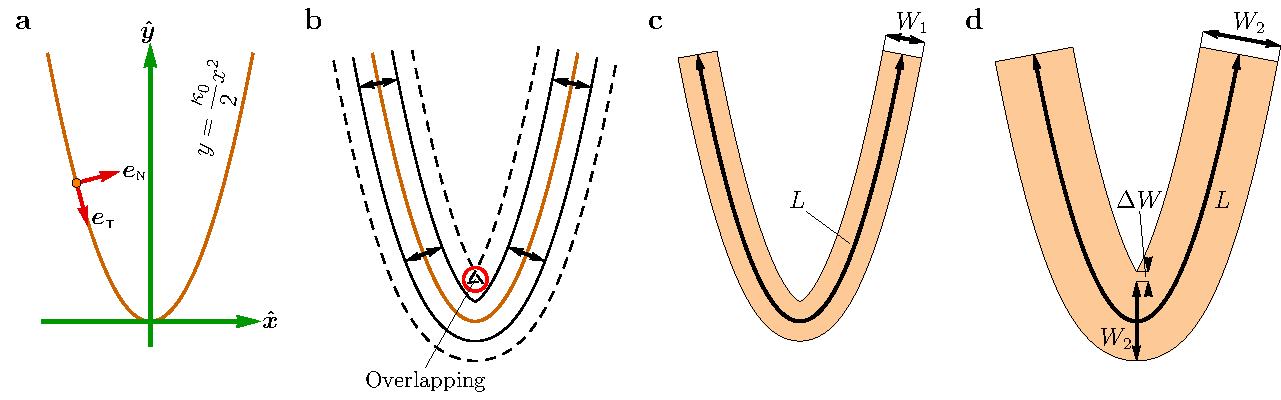
\includegraphics[width=0.9\linewidth]{fig_stripe_construction.pdf}
	\end{center}
	\caption{\textit{Geometrical construction of a parabolic stripe.}~(a), One-dimensional parabolic wire in a Cartesian frame of reference.~(b), Schematic picture of a parabolic stripe geometry construction from one-dimensional wire expansion along the normal direction $\vec{e}_\textrm{N}$.~(c) and (d), Show the resulting stripe geometries with two different widths $W_1$ and $W_2=2 W_1$, respectively. Local widening in the apex area of the parabolic stripe is indicated by $\Delta W$.}
	\label{fig:Parabola_stripe_geometry}
\end{figure*}	

\subsection{Lithographic methods}

Standard lithographic techniques combined with thin film deposition represent the first group of methods, that allow to fabricate two-dimensional curved magnetic objects. One of the most developed techniques among this group is Electron Beam Lithography (EBL) method, which allows to ensure shape retention of the patterned geometry and achieve high spatial resolution down to dozens of nanometers. A typical EBL system contains a precise emission source of electrons and necessary optics for the control and focusing of electron beam. The predetermined shape of the object is drawn in a electron-sensitive resist, whose solubility is changing under the electron beam exposure. This enables it selective removal of either the exposed (positive resist), or non-exposed (negative resist) regions of the resist by immersing it in a chemical developer. The remaining parts of the resist are using either for filling the remaining spaces between them with required material composition, or as a protection of the initially deposited layers from ion-beam etching. The resulting nanostructure could be revealed by removing the remaining resist in a specific solvent. This approach provided the opportunity to study magnetic processes in curved nanostripes~\cite{Lewis09,Nahrwold09,Glathe12} and nanorings~\cite{Klaui03a,Klaui05a,Klaui08,Richter16,Mawass17}  to address DW dynamics and automotion~\cite{Mawass17} for prospective memory~\cite{Hayashi07,Parkin08,Parkin15} and logic~\cite{Allwood02,Allwood04,Allwood05,Hrkac11} devices, as well as the concept of magnon-based processing of binary data~\cite{Schneider08,Lee08e,Vogt12,Vogt14,Chumak15}.


\subsection{Ion-induced methods}

\textit{Direct 2D writing} through the irradiation of B2-A2 phase alloys (e.g. FeAl alloy~\cite{Bali14}) allows to reach the element spatial resolution at the same or better level than lithography-based approaches. This method is based on thin films that are paramagnetic after preparation (B2 phase), but obtain ferromagnetic order after the irradiation due to the induced chemical disorder (A2 phase). As shown recently~\cite{Nord19}, using He$^{+}$ or Ne$^{+}$ irradiation in He-ion microscope it is possible to write into FeAl flat curvilinear magnetic nanostructures with a 2~nm precision.

%/-----------------------------------------------------------------------------------------
%
%Recent progress in material science enabled the appearance of various microscale additive manufacturing technologies, that provide the ability to build 3D curvilinear geometries that are not limited by the conventional lithographic or specific layer growth techniques~\cite{Hirt17}. One of the most prominent techniques of additive manufacturing of magnetic materials is focused electron-beam induced deposition (FEBID)~\cite{Teresa16,Huth18,Fernandez-Pacheco20} which in the recent years has reached a high level of maturity for the fabrication of complex-shaped 3D nano-architecures \cite{Keller18,Winkler19,Skoric20,Sanz-Hernandez20,Hunt20}. FEBID is based on the beam-induced dissociation of precursor organic molecules with the resulting non-volatile leftovers, that form a predetermined curvilinear geometry. The resulting self-standing magnetic geometries could be of any complex shape~\cite{Fernandez17}: self-standing magnetic nanostripes~\cite{Sanz-Hernandez17}, see Fig.~\ref{Fig:Experimental_figs_1}(g), nanoscale double-helix structures~\cite{Sanz-Hernandez20}, nano-cubes with nano-trees~\cite{Keller18,Mamoori18,Huth18} and nano-amphora~\cite{Huth20}. The two-photon lithography is another additive technology that allows to create sub-$\mu$m size self-standing curvilinear objects of various shapes that could be covered with magnetic materials~\cite{Williams18,Sahoo18,May19,Hunt20}, see Fig.~\ref{Fig:Experimental_figs_1}(h). This enables ``writing'' of almost arbitrary geometries and magnetic materials, which leads to the rapid prototyping of complex magnetic curvilinear geometries. 


\section{Characterization}\label{sec:characterization}

Magnetic characterization of flat curved structures utilizes the different methods, that could be generalized in the following groups:

\subsection{Magnetometry techniques}

This methods rely on measurements of magnetic responses from the curvilinear structures. Firstly, to this group should be included \textit{integral magnetometry} techniques, that provide the magnetic responses over the large-scale area and include the standard superconducting quantum interference device (SQUID) magnetometry, vibrating sample magnetometry (VSM) and magneto-optic Kerr effect (MOKE) magnetometry~\cite{Streubel12b,Streubel13c,Streubel14,Ueltzhoeffer16,Hunt20}, that recently was improved for high-precision analysis of curvilinear structures by utilizing dark-field MOKE magnetometry~\cite{Sanz-Hernandez17}, see Fig.~\ref{Fig:Experimental_figs_2}(a).

In addition to the integral methods, there is a group of \textit{local magnetometry} techniques  of the individual object, that retrieve both the spatial distribution of the stray fields and magnetic properties. This group includes dynamic cantilever-based~\cite{Degen09,Weber12,Mehlin18,Braakman19} (Fig.~\ref{Fig:Experimental_figs_2}(b)) and nano-SQUID magnetometries~\cite{Vasyukov18} (Fig.~\ref{Fig:Experimental_figs_2}(c)). Here it should be referred the scanning reconfigurable magnetic force microscopy (MFM)~\cite{Kazakova19,May19,Corte-Leon19}, that allows to quantify the 3D magnetization pattern of a magnetic nanoobject from a 2D data~\cite{Vock14}, and micro-Hall magnetometry that was applied for magnetic characterization of complex-shapes FEBID nanostructures~\cite{Keller18,Mamoori18} (Fig.~\ref{Fig:Experimental_figs_2}(d)). 

\begin{figure*}
	\centering
	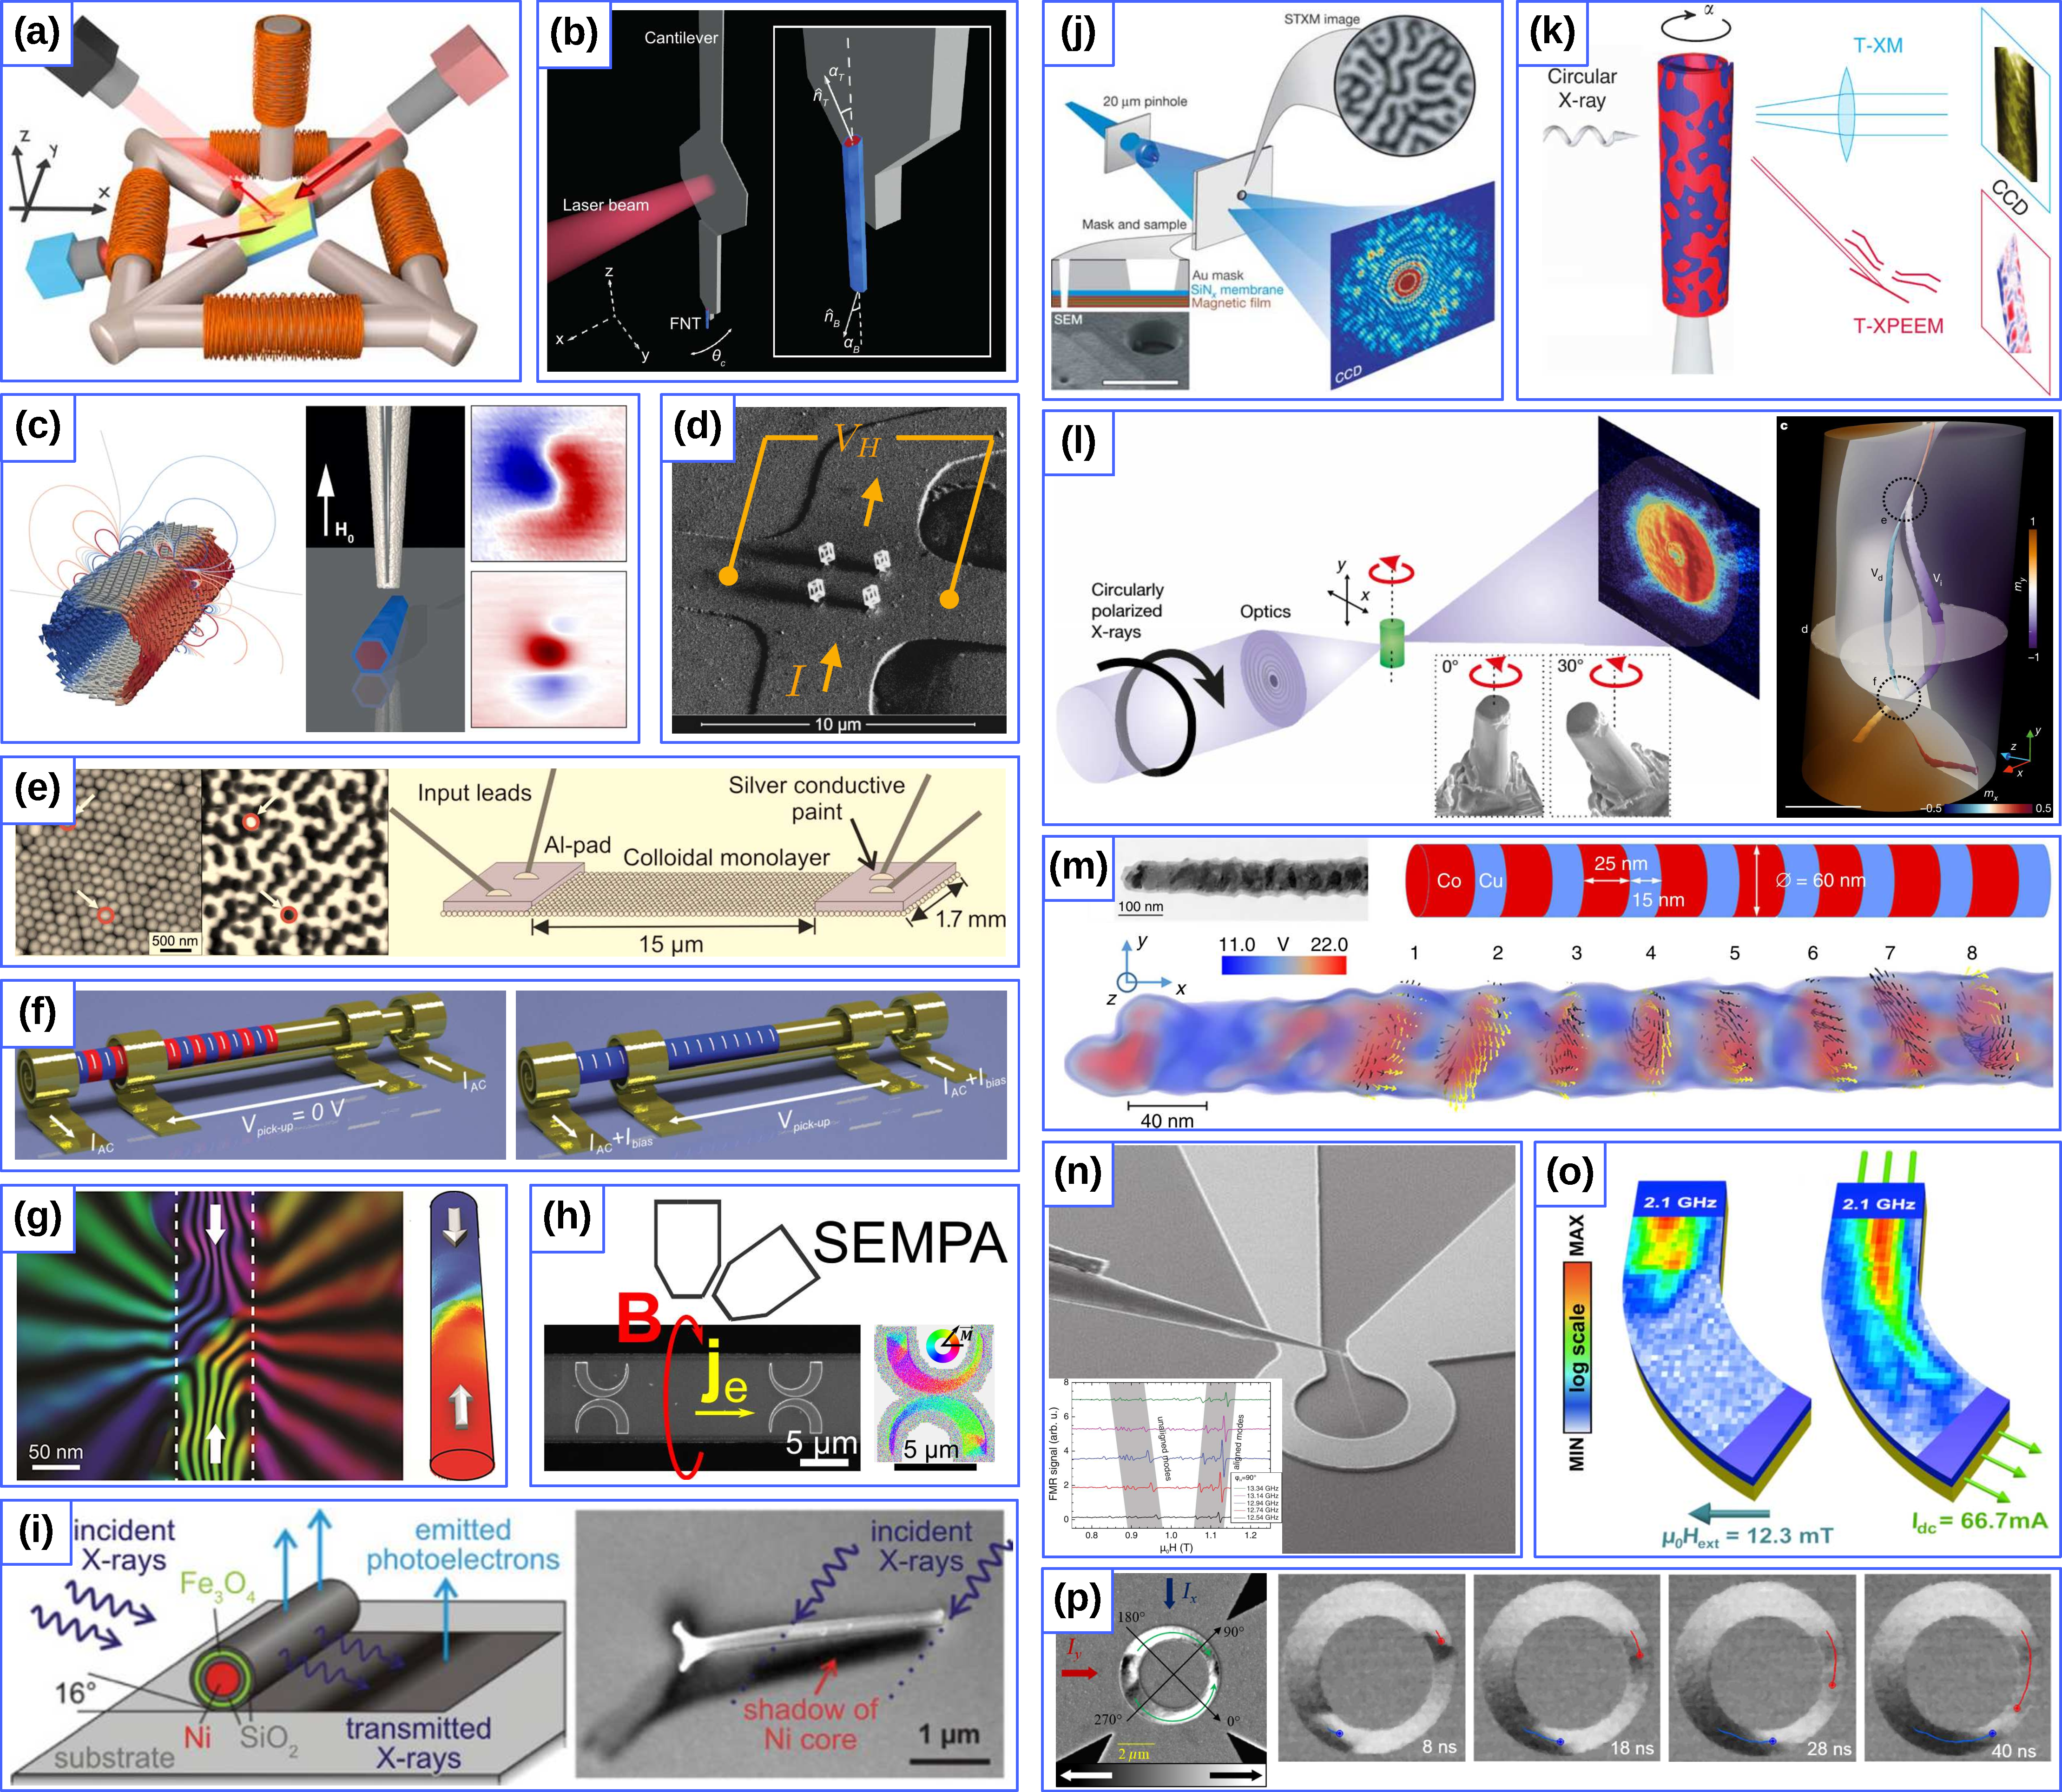
\includegraphics[width=0.97\linewidth]{fig_characterization.pdf}
	\caption{\textbf{Advanced characterization techniques for curvilinear nanomagnets.} \textbf{(a)} Schematics of dark-field MOKE. Adapted with permission from~\cite{Sanz-Hernandez17}. \textbf{(b)} Dynamic cantiliver-based magnetometry tip with magnetic nanotube at the end. Adapted with permission from~\cite{Mehlin18}. \textbf{(c)} Nano-SQUID tip and reconstructed stray field of hexagonal magnetic nanotube. Adapted with permission from~\cite{Vasyukov18}. \textbf{(d)} Micro-Hall cross setup with nanocubes. Adapted with permission from~\cite{Mamoori18}. \textbf{(e)} Sketch of AMR measurements on self-assembled magnetic nanoparticles. Adapted with permission from~\cite{KimlingnMoser10}. \textbf{(f)} Schematics of an integrated GMI sensor operation. Adapted with the permission from~\cite{Karnaushenko15a}. \textbf{(g)} Electron holography of a DW in Ni nanocylinder. Adapted with permission from~\cite{Biziere13}. \textbf{(h)} Sketch of SEMPA setup and color-coded image from flat curvilinear structures. Adapted with permission from~\cite{Schoenke20}. \textbf{(i)} XMCD-PEEM technique for 3D magnets with shadow contrast reconstruction. Adapted with permission from~\cite{Kimling11}. \textbf{(j)} (i) X-ray spectro-holography. Adapted with permission from~\cite{Eisebitt04}.
	\textbf{(k)} Concept of MXT based on a combination of STXM and XMCD-PEEM techniques for the 3D magnets. Adapted with permission from~\cite{Streubel15a}. \textbf{(l)} Hard X-Ray magnetic tomography setup based on ptychographic scans of a sample. Adapted with permission from~\cite{Donnelly17}.	\textbf{(m)} Holographic vector field electron tomography of 3D nanomagnets. Adapted with permission from~\cite{Wolf19}. \textbf{(n)} FMR measurements of a magnetic nanowire in $\Omega$-shaped resonator. Adapted with permission from~\cite{Lenz19}. \textbf{(o)} BLS intensity distribution of spin waves in a curved stripe. Adapted with permission from~\cite{Vogt12}. \textbf{(p)} Asymmetric ferromagnetic ring and STXM snapshots of automotive DWs motion. Adapted with permission from~\cite{Mawass17}.} 
	\label{Fig:Experimental_figs_2}
\end{figure*}

\subsection{Transport techniques}

This group of techniques provide the insight into the charge and spin transport properties of magnetic materials. These techniques include the group of magneto-sensitive transport-based electrical measurements, that employs: anisotropic magnetoresistance (AMR) effect for nanotubes~\cite{Rueffer12,Zimmermann18}, monolayer of magnetic spherical caps~\cite{KimlingnMoser10} (Fig.~\ref{Fig:Experimental_figs_2}(e)), ferromagnetic microhelices~\cite{Maurenbrecher18} and nanomembranes~\cite{Moench11,Schumann12,Muller12}; giant magnetoresistive (GMR) effect for nanomembranes~\cite{Mueller12}; giant magnetoimpedance (GMI) effect~\cite{Karnaushenko15a} Fig.~\ref{Fig:Experimental_figs_2}(f); current-induced spin torques~\cite{Schoebitz19}. 

\subsection{Magneto-sensitive visualization techniques}

A valuable information about the magnetization textures of curvilinear objects can be obtained by magneto-sensitive visualization techniques, that provide access to complex magnetization patterns on curved magnetic systems. These techniques include \textit{scanning-probe methods}, e.g. MFM, that provide a spatial resolution up to 50~nm for curved nanoobjects~\cite{Ulbrich06,Makarov07,Makarov08,Makarov09,Schulze10,Albrecht12,Nguyen15,Streubel16,Ball17,May19}; MOKE microscopy~\cite{Streubel12b,Streubel13c,Streubel14,Ueltzhoeffer16,Hunt20}, that recently was enabled for pump-probe time-resolved measurements of micro-tetrapod geometries~\cite{Sahoo18}; electron-based methods, including Lorentz transmission electron microscopy (TEM)~\cite{Phatak12,Phatak11} with its extension to electron holography, that allows to perform the detail static reconstruction of magnetic textures in flat~\cite{Klaeui05,Nord19} and 3D~\cite{Biziere13,Phatak14,Phatak20} curved geometries, see Fig.~\ref{Fig:Experimental_figs_2}(g); scanning electron technique with polarization analysis~(SEMPA)~\cite{Schoenke18}, that is suitable for imaging flat curved magnetic geometries~\cite{Klaui05,Schoenke20}, see Fig.~\ref{Fig:Experimental_figs_2}(h); X-ray-based visualization methods, including X-ray magnetic circular dichroism photoelectron emission microscopy (XMCD-PEEM)~\cite{Streubel15c,Streubel15,Streubel16,Volkov19,Volkov19c}.  

While these methods are limited to the analysis of simple magnetic geometries, the visualization of complex 3D shape geometries requires the utilization of the tomographic-based approaches. Thus, MOKE microscopy~\cite{Streubel14}, that recently was enabled for tomography-like screening of bulk samples~\cite{Schaefer20}; XMCD-PEEM was successfully extended to image interior magnetization textures of complex curved magnetic nanoobjects by using transmission shadow contrasts~\cite{Kimling11,Streubel12,Streubel12b,Streubel14a,DaCol14,Stano18a,Wartelle18,Schoebitz19,Wartelle19}, see Fig.~\ref{Fig:Experimental_figs_2}(i). X-ray spectro-holography~\cite{Eisebitt04} could be also utilizes for the characterization of 3D curved magnetic nanostructures (Fig.~\ref{Fig:Experimental_figs_2}(j)), e.g. magnetically capped nanospheres~\cite{Guenther10}. Full field X-ray microscopy, that combines magnetic transmission
soft X-ray microscopy (MXTM) with XMCD-PEEM, was successfully applied to realize the concept of soft X-ray magnetic tomography (MXT)~\cite{Streubel15a}, see Fig.~\ref{Fig:Experimental_figs_2}(k). Complementary, hard X-ray magnetic tomography with ptychographic scans potentially allows for 10 nm resolution of 3D magnetic textures~\cite{Donnelly17}, see Fig.~\ref{Fig:Experimental_figs_2}(l). The electron holography is extended to holographic vector field electron tomography~\cite{Wolf13,Wolf19}, see Fig.~\ref{Fig:Experimental_figs_2}(m), that allows to reconstruct 3D magnetic textures with a sub 10~nm resolution. 

\subsection{Dynamic magnetization methods}

Other methods, that rely on time domain and provide input on magnetization characterization are dynamic methods. These techniques include the ferromagnetic resonance (FMR) methods~\cite{Liedke13}, whose sensitivity for the study of curved magnetic objects could be substantially improved by utilizing microresanator loops~\cite{Lenz19}, see Fig.~\ref{Fig:Experimental_figs_2}(n). Another valuable dynamic measurement method is Brillouin light spectroscopy (BLS)~\cite{Demokritov01}, that recently was improved by using high-sensitive BLS microscopy~\cite{Vogt12,Vogt14,Schultheiss19}, see Fig.~\ref{Fig:Experimental_figs_2}(o). Also, it should be mentioned the possibility to perform dynamic magnetic imaging using scanning transmission X-ray microscope (STXM)~\cite{Wintz11,Streubel15,Streubel15d,Wintz16,Woo16,Zimmermann18,Sluka19}, see Fig.~\ref{Fig:Experimental_figs_2}(p).



%These techniques include the scanning-probe near-field methods, that are represented by: scanning reconfigurable magnetic force microscopy (MFM)~\cite{Kazakova19,May19,Corte-Leon19}, nano-superconducting quantum interference device magnetometry~\cite{Vasyukov18} and dynamic cantilever magnetometries~\cite{Degen09,Weber12,Mehlin18,Braakman19}. These methods allow to retrieve the magnetic properties and magnetization configuration from the demagnetizing fields of curvilinear structures. To the magnetometry techniques should be also included the group of magneto-sensitive transport-based electrical measurements, that employs: anisotropic magnetoresistance (AMR) effect for nanotubes~\cite{Rueffer12,Zimmermann18}, monolayer of magnetic spherical caps~\cite{KimlingnMoser10}, ferromagnetic microhelices~\cite{Maurenbrecher18} and nanomembranes~\cite{Moench11,Schumann12,Muller12}; giant magnetoresistive (GMR) effect for nanomembranes~\cite{Mueller12}; giant magnetoimpedance (GMI) effect~\cite{Karnaushenko15a}; micro-Hall magnetometry that was applied for magnetic characterization of complex-shapes FEBID nanostructures~\cite{Keller18,Mamoori18}; current-induced spin torques~\cite{Schoebitz19} and spin-orbit torques~~\cite{Miron10,Miron11a,Garello13,Manchon19}; magneto-optic Kerr effect (MOKE) magnetometry~\cite{Streubel12b,Streubel13c,Streubel14,Ueltzhoeffer16,Hunt20}, that recently was improved for high-precision analysis of curvilinear structures by utilizing dark-field MOKE magnetometry~\cite{Sanz-Hernandez17}.




% To these techniques should be also referred the mentioned above \textit{scanning-probe methods}, including MFM, that provide a spatial resolution up to 50~nm for curved nanoobjects~\cite{Ulbrich06,Makarov07,Makarov08,Makarov09,Schulze10,Albrecht12,Nguyen15,Streubel16,Ball17,May19}. MOKE microscopy~\cite{Streubel14}, that recently was enabled for tomography-like screening of bulk samples~\cite{Schaefer20} and pump-probe time-resolved measurements of micro-tetrapod geometries~\cite{Sahoo18}. The high-resolution magnetic imaging of curved geometries is achieved by means of different X-ray-based visualization methods, including X-ray magnetic circular dichroism photoelectron emission microscopy (XMCD-PEEM)~\cite{Streubel15c,Streubel15,Streubel16,Volkov19,Volkov19c}, that was successfully extended to image interior magnetization textures of complex curved magnetic nanoobjects by using transmission shadow contrasts~\cite{Kimling11,Streubel12,Streubel12b,Streubel14a,Wartelle18,Schoebitz19,Wartelle19}, see Fig.~\ref{Fig:Experimental_figs_2}(b), and subsequently modified to the concept of soft X-ray magnetic tomography (MXT)~\cite{Streubel15a}, see Fig.~\ref{Fig:Experimental_figs_2}(c), and hard X-ray magnetic tomography with ptychographic scans potentially allows for 10 nm resolution of 3D magnetic textures~\cite{Donnelly17}, see Fig.~\ref{Fig:Experimental_figs_2}(a). It should be mentioned also the possibility to utilize the X-ray spectro-holography~\cite{Eisebitt04} for the characterization of microscopic magnetically capped nanospheres~\cite{Guenther10}. Another valuable imaging techniques are electron-based methods, including scanning electron technique with polarization analysis~(SEMPA)~\cite{Schoenke18}, that is suitable for imaging flat curved magnetic geometries~\cite{Klaui05,Schoenke20}, Lorentz transmission electron microscopy (TEM)~\cite{Phatak12,Phatak11} with its extension to electron holography, that allows to perform the detail static reconstruction of magnetic textures in flat~\cite{Klaeui05,Nord19} and 3D~\cite{Phatak14,Phatak20} curved geometries, and its further extension to holographic vector field electron tomography~\cite{Wolf13,Wolf19}, see Fig.~\ref{Fig:Experimental_figs_2}(d), that allows to reconstruct 3D magnetic textures with a sub 10~nm resolution.


%The \textbf{characterization of magnetic responses} from 3D curvilinear objects utilizes (I) a high-resolution magneto-sensitive visualization techniques, that enable a direct reconstruction of the magnetization distribution in 3D object,  and (II) advanced magnetometry techniques, that indirectly infer the magnetic configuration of nanosctructure, as demonstrated in Fig.~\ref{Fig:Experimental_figs_2}. The first type of techniques is based on the high-resolution vector tomography, e.g. the hard X-Ray magnetic tomography with ptychographic scans potentially allows for 10 nm resolution of 3D magnetic textures~\cite{Donnelly17}, see Fig.~\ref{Fig:Experimental_figs_2}(a). Soft X-Ray magnetic circular dichroism photoelectron emission microscopy (XMCD-PEEM) was successfully applied to image interior domain patterns in nanorods relying on a transmission shadow contrast~\cite{Kimling11}, see Fig.~\ref{Fig:Experimental_figs_2}(b). This method was modified to the concept of soft X-ray magnetic tomography (MXT)~\cite{Streubel15a}, see Fig.~\ref{Fig:Experimental_figs_2}(c). Another valuable tomographic method, that allows to reconstruct magnetic textures with a sub 10 nm resolution, is holographic vector field electron tomography~\cite{Wolf13,Wolf19}, see Fig.~\ref{Fig:Experimental_figs_2}(d). It should be mentioned also the possibility to utilize the X-ray spectro-holography~\cite{Eisebitt04} for the characterization of microscopic magnetically capped nanospheres~\cite{Guenther10}. 

%The second type of experimental methods relies on the novel magnetometry techniques, that rely on the indirect measurements of magnetic responses from the curvilinear structures. There are optical, electrical and near-field high-sensitive magnetometry methods. The first type of magnetometry techniques is based on the magnetooptical Kerr effect (MOKE) and Brillouin light spectroscopy (BLS)~\cite{Demokritov01} methods. Recently, the standard MOKE was developed for high-precision analysis of curvilinear structures by utilizing dark-field MOKE magnetometry~\cite{Sanz-Hernandez17}, pump-probe time-resolved MOKE measurements~\cite{Sahoo18}  and tomography-like MOKE screening of bulk samples~\cite{Schaefer20}, while the convenient BLS method was improved by using high-sensitive BLS microscopy~\cite{Vogt12,Vogt14,Schultheiss19}. The group of electrical magnetometry techniques is based on the resistance measurements of magnetic samples in external field, that employs magnetoresistance~\cite{KimlingnMoser10,Maurenbrecher18}, micro-Hall~\cite{Keller18,Mamoori18} effects and current-induced spin-orbit torques in magnetic systems~\cite{Miron10,Miron11a,Garello13,Manchon19}. The near-field magnetometry method are represented by a scanning reconfigurable magnetic force microscopy (MFM)~\cite{Kazakova19,May19,Corte-Leon19}, nano-superconducting quantum interference devices~\cite{Vasyukov18} and dynamic cantilever magnetometries~\cite{Mehlin18}. 

\section{Conclusions}\label{sec:conclusions}

some text

\bibliographystyle{splncs}
\bibliography{soliton}
\end{document}
